\chapter{Analyzing, explaining, and teaching vocabulary} \label{ch:vocabulary}

\epigraph{Language is an unfinished business. Words come and go, taking their chances like everyone else.}{}

\section{Introduction} \label{sec:intro}

For many people, language is all about words. It's not that they discount grammar, but words are just so salient, and there are so very many of them. Words form a huge part of language learning, and for students, they often feel like one of the more concrete aspects of English to master. There's a clear sense of progress as new words are acquired. The sheer volume of vocabulary to be learned, though, presents challenges for teachers in terms of selection, presentation, and practice.

This chapter digs into various aspects of vocabulary itself, along with teaching and learning strategies. We'll examine:

\begin{itemize}
\item How words are constructed (morphology)
\item What constitutes a ``word'' and different ways to count vocabulary
\item How much vocabulary learners need, and which words to prioritize
\item The frequency distribution of words in English
\item Teaching and learning vocabulary
\end{itemize}

Understanding these aspects can help you approach vocabulary instruction more effectively. While grammar and pronunciation have their own challenges, vocabulary often requires significant time and effort from learners due to its sheer quantity. There are thousands of words to learn, each with varying degrees of importance and utility. Some common approaches to vocabulary teaching and learning aren't as efficient as others.

By the end of this chapter, you'll have a clearer picture of how to approach vocabulary instruction. You'll be better equipped to make informed choices about which words to prioritize, how to present them, and how to help your students retain and use new vocabulary effectively. We'll emphasize practical, evidence-based strategies that maximize learning efficiency and consider the opportunity cost of vocabulary choices.

We begin by examining the building blocks of vocabulary: morphemes and word formation. This foundation will inform our subsequent discussions on vocabulary size, selection, and instruction techniques.

\section{The Four Strands of Vocabulary Learning} \label{sec:four-strands}

While this chapter focuses primarily on explicit vocabulary instruction (what Nation calls ``language-focused learning''), it's crucial to understand that vocabulary acquisition occurs through four complementary strands:

\begin{enumerate}
    \item \textbf{Meaning-focused input:} Learning vocabulary through listening and reading
    \item \textbf{Meaning-focused output:} Learning through speaking and writing
    \item \textbf{Language-focused learning:} Direct study of vocabulary
    \item \textbf{Fluency development:} Practising with known vocabulary (see Chapter \ref{ch:fluency})
\end{enumerate}

The bulk of vocabulary learning should occur through meaning-focused input and output, with language-focused learning serving as a complement to these primary channels. This principle applies not only to vocabulary but to all aspects of language learning including grammar, morphology, pronunciation, and spelling.

Each strand should receive roughly equal time in a well-balanced language program. This chapter emphasizes language-focused learning for two reasons. First, it's where teachers have the most direct control and where principled selection of teaching targets is most crucial. Second, explicit vocabulary instruction can be particularly beneficial in early stages of language learning, to bootstrap learners to a point where they have sufficient vocabulary to participate extensively in meaning-focused activities \citep[CITATION NEEDED]{}.

\section{What's a word}\label{sec:what-is-a-word}

For many people, words are the essence of language. They're the building blocks we use to construct meaning, the units we count when measuring text length, and often the focus of language learning efforts. Yet defining exactly what constitutes a ``word'' is trickier than it might seem at first glance.

In this section, we'll explore the complexities of words from several angles:

\begin{itemize}
    \item Semantic vs syntactic notions of a word
    \item How words are formed and change (morphology)
    \item Why understanding word formation matters for vocabulary learning
    \item Key affixes that can expand your students' word knowledge efficiently
    \item Different ways of conceptualizing words for various purposes
\end{itemize}

By the end, you'll have a clearer picture of what we mean when we talk about ``words'' in English, and how this understanding can inform your approach to vocabulary instruction.

\subsection{Semantic and syntactic notions of words}

When discussing words, it's useful to distinguish between the semantic and syntactic perspectives. They don't always coincide, and sometimes misunderstandings are simply due to a lack of a shared perspective.

From a semantic standpoint, a word is a unit of meaning. This view focuses on the conceptual content rather than grammatical behavior. Dictionaries typically reflect this perspective, treating semantically unified strings such as \href{https://www.ldoceonline.com/dictionary/have-a-go}{\textit{at the moment}}, meaning `now' as single entries even when they consist of multiple syntactic parts. A prime example of this is the treatment of so-called ``phrasal verbs''.\footnote{Phrasal verbs like \textit{put up with} are often only phrases in the traditional sense of `a group of words' and not in the technical sense of a `a syntactic head and its dependents'.} Consider the case of \textit{give up}:

\ea \textit{I decided to \uline{give up} smoking.}
\z

\noindent Semantically and lexicographically, \textit{give up} functions as a single unit of meaning `stop doing or trying something'. You'd find it as one entry in a dictionary, despite its two-part composition.

Syntactically, though, we often need to treat the components of such expressions as separate words. This is the view we've been employing in our discussions of lexical categories in earlier chapters. From this angle, \textit{give} and \textit{up} are distinct syntactic units, a verb and a preposition, as evidenced by their ability to be separated in certain constructions:

\ea
\ea \textit{I \uline{gave up} smoking last year.}
\ex \textit{I \uline{gave} it \uline{up} last year.}
\z\z

This syntactic flexibility demonstrates why, grammatically, we often need to consider \textit{give} and \textit{up} as separate words, even when it takes both to convey the intended meaning.

Both perspectives are valid, but you should try to be aware of which is in play at any given time.

While these different notions of words help us understand their behavior in phrases and sentences, there's another crucial aspect to consider: how words themselves are formed and how they change. This brings us to the study of morphology.

\subsection{Morphology} \label{sec:morphology}

\textsc{Morphology} is the study of how words change their form or category. For example, the fact that you can add \textit{--ly} to the adjective \textit{happy} and get the adverb \textit{happily} is a morphological fact. As is the fact that you can get the noun \textit{run} from the verb \textit{run} without changing anything at all. Some languages are rich in morphology, but English is pretty simple, especially when it comes to the morphology that English-language learners need to know.

Word can be formed of \textsc{bases} and \textsc{affixes}. All words contain at least one base, and most bases are words in their own right. For example, the base of \textit{happiness} is \textit{happy}, which is obviously a word. In contrast, \textit{--ness} is an affix, which depends on a base. This is very much like the syntactic idea of heads (Section \ref{sec:head}) and dependents (Section \ref{sec:Dep}). But just as some syntactic heads, such as the verb \textit{helped}, can't form a sentence on their own, some bases cannot stand alone as words. One example is \textit{dur}, as in \textit{durable} or \textit{duration}. \textit{Dur} is never a word on its own, but nor does it combine with any free bases.

There are also special bases called \textsc{combining forms}. These include examples such as \textit{bio} and \textit{ology}, which combine to form words such as \textit{biology}. Combining forms usually combine with each other, but sometimes they can combine with a free base, as in \textit{bio-mechanical}.

\subsection{What's morphology doing in a chapter on vocabulary?}

In English, it's often the case that, even if you've never seen a word before, you can work its meaning out if you know something about morphology. For example, you've probably never seen the word \textit{decountrify}, but you can probably guess what it might mean because you know \textit{de--}, \textit{country}, and \textit{--ify}. It's the same for your English-language learners.

\begin{tcolorbox}[title=Self-check, colback=white]

    Notice here that I said, ``your English-language learners.'' In a footnote to Section \ref{sec:pronouns}, I said we'd call words like \textit{your} \textsc{possessive pronouns} as long as you'd remember that such words don't always mark possession. Unfortunately, some people are confused about this point, and so \href{https://twitter.com/search?q=%22my%20students%22%20possessive&src=typed_query&f=top}{they object} to teachers' use of expressions like \textit{my students}. Don't be fooled. \textit{My students} doesn't mean that you own or possess the students any more than your pet's vet is owned by your pet or \textit{the problem's causes} means the problem somehow possesses its causes. \textit{My} can mean that, but that's not the only thing it can mean (see Section \ref{sec:monosemy}). In cases like \textit{my students}, it is marking 
    
    \begin{quote}
        a noun denoting something with which one has a less immediate or definite relation (such as a target or objective, a field of study, an honour or award, or an academic qualification).\hfill\citep{oed_my}
    \end{quote}
            
    To be clear, there is nothing inherently offensive about saying \textit{my students}.
\end{tcolorbox}

If your students know \textit{industry}, along with some common suffixes, then they get \textit{industrialization} ``for free'', as it were.

Fortunately, there aren't even that many common affixes to learn, and if your students speak another European language, they may already be familiar with many or all of them. 

\subsection{Some important affixes} \label{sec:derivation}

According to \textit{The Longman grammar of spoken and written English} \citep[401]{Biber1999}, the following affixes stand head and shoulders above others of their category in terms of their frequency in their 40-million-word corpus. It's worth teaching them to your students. Of course, there are many other affixes, but they apply to so few words that it's really not worth your students' time to study them. This principle of cost-benefit analysis is one we'll come back to in Section \ref{sec:word-frequency}.

\subsubsection*{Verb-forming suffixes}
Some suffixes change a word into a verb. For example, to describe somebody's character is to \textit{characterize} them. The verb \textit{characterize}, then, is formed by adding the verb-forming suffix \textit{--ize} to the noun \textit{character}. The following are the most common verb-forming suffixes, occurring in roughly 20--170 verbs each: \textit{--ize}/\textit{ise,} \textit{--en}, \textit{--ate}, and \textit{--}(\textit{i})\textit{fy}. 

\subsubsection*{Verb-changing prefixes}
While the suffixes tend to change nouns or adjectives into verbs, the prefixes below change the meaning of the verb without changing its lexical category. For example, if you \textit{overdo} something, you do it too much. But both \textit{do} and \textit{overdo} are verbs. The most common of these prefixes~-- the ones your students should know about~-- are: \textit{re--}, \textit{over--}, \textit{un--}, \textit{mis--}, and \textit{out--} \citep[400]{Biber1999}.

\subsubsection*{Noun-forming suffixes}
Just as there are verb-forming suffixes that change adjectives and nouns into verbs, there are noun-forming suffixes that change adjectives and verbs into nouns. For example, \textit{openness} is the adjective \textit{open} + the suffix \textit{--ness}. For nouns, the list is slightly longer than the list for verbs, especially if your students are learning English for academic purposes. It includes, from most to least productive, \textit{--tion}, \textit{--ism}, \textit{--ity}, \textit{--ness}, \textit{--ism}, \textit{--ment}, \textit{--ant}, \textit{--ship}, \textit{--age}, and \textit{--ery}.

There are about 2,000 nouns ending in \textit{--tion} in the Longman grammar's corpus, and only about 50 ending in \textit{--ery}. This dramatic difference in frequency between the most frequent and even slightly less frequent elements is a fundamental pattern we'll see repeated across various aspects of vocabulary (e.g., in Section \ref{sec:word-frequency}).

Again, there are many other affixes in English, but most appear only in a few words and have a poor return for study time invested.

The same is true of most combining forms. For example, \textit{sta} means `stand, set down, make or be firm', and appears in quite a few words, including those in (\ref{ex:sta-words}).
\ea\textit{constant}, \textit{contrast}, \textit{destination}, \textit{distant}, \textit{estate}, \textit{instant}, \textit{prostitute}, \textit{restore}, \textit{stage}, \textit{system}, \textit{understand}\label{ex:sta-words}
\z
\noindent But the connection to \textit{sta} is mostly obscure, unhelpful, or both. For instance, it's hard to imagine how knowing about \textit{sta} would allow a typical student to work out the meaning of any of the words in (\ref{ex:sta-words}). For this reason, it's rarely helpful to spend time teaching bases like this.

\subsection{Inflectional morphology}

The morphology discussed in Section \ref{sec:derivation} is all called \textsc{derivational morphology} and deals with how words are formed. There are, however, a number of suffixes that really don't form new words, change a word's lexical category, or result in a change in meaning, but which mark grammatical systems such as tense, number, comparison, etc. The possessive \textit{'s} is one. There's also the \textit{--s}, \textit{--ed}, and \textit{--ing} suffixes that attach to verbs (see Section \ref{sec:verb-forms}), the plural \textit{--s} that attaches to nouns, and the \textit{--er} and \textit{--est} suffixes on adjectives and adverbs. They don't really belong in a chapter on vocabulary though, so I'll dispense with them simply by acknowledging their existence and saying that they're involved in what we call \textsc{inflectional morphology}.


\subsection{Word families, lemmas, shapes, and tokens}\label{sec:family-lemma-shape-token}

As we've just seen, words in English can take various forms through inflection and derivation. This variability makes the seemingly simple task of counting words surprisingly complex. How do we account for words like \textit{wide}, \textit{wider}, and \textit{width}? Are they separate words, or variations of the same word? To address these complexities, linguists and language educators use several different ways of grouping and counting words, each serving different purposes: word families, lemmas, shapes (also known as types), and tokens.

\paragraph*{Word families:}A \textsc{word family} includes a base word and all its inflectionally and derivationally related words. All the words in the following list belong to a single word family, the \textit{wide} family: \textit{wide},
\textit{wider},
\textit{widest},
\textit{widely},
\textit{widen},
\textit{widens},
\textit{widened},
\textit{widening},
\textit{wideness},
\textit{widener},
\textit{wideners}, and
\textit{width}.\footnote{You could add \textit{widespread}, \textit{wide-ranging}, \textit{wide-eyed}, etc.}

\begin{tcolorbox}[title=Word Families and Morphological Development] \label{sec:word-family-debate}

Recent debates have highlighted that the size and composition of word families isn't fixed but relates to learners' mastery of morphology (e.g., \cite{Webb2021}). A word family includes a base word plus its inflected and derived forms, but which derived forms belong to a family depends on the learner's knowledge of English morphology.

~~~~For instance, for a beginner, \textit{industry} and \textit{industrious} might belong to separate families, while an advanced learner would recognize them as part of the same family. Even expert users of English may not recognize etymologically related pairs like \textit{abyss}/\textit{abysmal} as belonging to the same family, and for teaching purposes, such distant relationships are rarely useful. This understanding has implications for:


\begin{itemize}
    \item How we count vocabulary size
    \item Which words we consider ``known''
    \item When to teach derived forms explicitly
    \item How we assess vocabulary knowledge
\end{itemize}

~~~~As learners develop their understanding of English, their ability to recognize related words increases, effectively expanding their word families.
\end{tcolorbox}

\begin{tcolorbox}[title=A Family Analogy]
\begin{itemize}
    \item \textbf{Word Family:} The extended \textit{Wide} clan
    \item \textbf{Lemmas:} Households within the clan
    \begin{itemize}
        \item The \textit{Wide} household (adjectives)
        \item The \textit{Widen} household (verbs)
        \item The \textit{Width} household (nouns)
    \end{itemize}
    \item \textbf{Shapes:} Individual family members
    \begin{itemize}
        \item E.g., \textit{Wide}, \textit{Wider}, \textit{Widest} in the \textit{Wide} household
    \end{itemize}
    \item \textbf{Tokens:} Each encounter with a family member
    \begin{itemize}
        \item Seeing Aunt Wide at a reunion and again at the store: 2 tokens
    \end{itemize}
\end{itemize}
\end{tcolorbox}


\begin{figure}[htbp]
\centering
\begin{forest}
for tree={
  grow'=east,
  font=\sffamily,
  text width=2cm,
  text centered,
  parent anchor=east,
  child anchor=west,
  edge={thick},
  l sep+=0.5cm,
  s sep+=0.1cm,
  rounded corners,
  draw
}
[{Word Family\\{\itshape wide}}
  [{Lemma\\{\itshape wide} (adj)}
    [{Shape\\{\itshape wide}}
      [{Token\\{\itshape wide}}]
      [{Token\\{\itshape wide}}]
    ]
    [{Shape\\{\itshape wider}}
      [{Token\\{\itshape wider}}]
    ]
  ]
  [{Lemma\\{\itshape widen} (verb)}
    [{Shape\\{\itshape widen}}
      [{Token\\{\itshape widen}}]
      [{Token\\{\itshape widen}}]
      [{Token\\{\itshape widen}}]
    ]
    [{Shape\\{\itshape widens}}
      [{Token\\{\itshape widens}}]
    ]
  ]
  [{Lemma\\{\itshape width} (noun)}
    [{Shape\\{\itshape width}}
      [{Token\\{\itshape width}}]
    ]
  ]
]
\end{forest}
\caption{\textit{Wide} family tree in a text where \textit{wide} occurs twice, \textit{wider} once, \textit{widen} three times, \textit{widens once}, and \textit{width} once. The other shapes, such as \textit{widest} and \textit{widening}, didn't occur in the text.}
\label{fig:wide-family-tree}
\end{figure}


\paragraph*{Lemmas:}The inflectionally related words belong to a single \textsc{lemma}. For example, the verb lemma \textit{widen} includes \textit{widen}, \textit{widens}, \textit{widened} (past tense), \textit{widened} (past participle), and \textit{widening}. I've included five lemmas in the \textit{wide} family: an adjective \textit{wide}, an adverb \textit{widely}, a verb \textit{widen}, and two nouns \textit{widener} and \textit{width}. Generally, a lemma is what you look up in the dictionary. If you want to know about the superlative adjective \textit{widest}, you look under the adjective lemma \textit{wide}. If you look at \textit{widest}, you may find no entry, or you may be redirected to \textit{wide}.

\paragraph*{Word shapes:}Each inflectional or derivational word form is a different \textsc{shape} (\textit{type} is another commonly used term). In the \textit{wide} lemma, there are three shapes: \textit{wide}, \textit{wider}, and \textit{widest}. The \textit{wide} family includes at least those in Figure \ref{fig:wide-family-tree}.

\paragraph*{Word tokens:}A \textsc{word token} is a single instance or occurrence of a word in a text or utterance. If an article is 800 words long, it has 800 tokens, even if 56 of those tokens are \textit{the}, for instance. Counting word tokens is the normal way of counting words for school assignments and publishing.

The reason we need these different ideas of a word is that they're all useful in different ways. 

If you want to know how many words a learner has learned, you're probably talking about word families. If somebody learned \textit{run}, for example, and they know something about English, then \textit{runs}, \textit{running}, and \textit{runners} all come ``for free''; they haven't really learned four words, but rather one word family. Similarly, if the teacher used members of the \textit{run} family in its various forms 12 times during the class and the students also read it 15 times, we don't want to say they've learned 27 words. So word families are helpful for thinking about vocabulary size.

But if you want to know about reading speed, you're counting tokens; if somebody says, ``I can read 160 words per minute,''  it doesn't matter how many of those words are repeated or even related. And, again, when a teacher says, ``write 500 words,' they mean word tokens.

As we saw above, what you look up in a dictionary is usually a lemma. If a dictionary says it has 180,000 words, it means 180,000 lemmas. Inside each lemma (e.g., verb \textit{run}), there are more forms (e.g., \textit{running}, \textit{ran}, etc.), but the dictionary doesn't include those in the number of words covered. On the other hand, it counts \textit{run} and and \textit{runner} as two words, even though they're in the same word family.

Finally, if you want to know how many different forms are included in a lemma or word family, you're asking about shapes. For example, the verb lemma \textit{go} has five shapes (\textit{go}, \textit{goes}, \textit{going}, \textit{went}, and \textit{gone}), but the lemma \textit{be} has many more shapes than any other verb (15 in fact!).

\begin{tcolorbox}[title=Exercise: Word Families and Lemmas, colback=white, colframe=blue!75!black, fonttitle=\bfseries]
1. For each of the following words, list at least three other words that belong to the same word family:

\begin{enumerate}
    \item \textit{happy}
    \item \textit{create}
    \item \textit{science}
    \item \textit{electric}
    \item \textit{politics}
\end{enumerate}

2. Identify the lemma(s) for each of the following words:

\begin{enumerate}
    \item \textit{running}
    \item \textit{better}
    \item \textit{mice}
    \item \textit{went}
    \item \textit{lives}
\end{enumerate}

3. Explain the difference between a word family and a lemma, using examples from your answers above.
\end{tcolorbox}

\begin{tcolorbox}[title=Searching for shapes and lemmas]
    If you're \href{https://www.english-corpora.org/coca/}{searching in COCA}, you usually just enter a word or string of words (e.g., \texttt{run} or \textit{run down}), and this will give you just the shape \textit{run} (every word spelled $\langle$run$\rangle$). But you can also enter \texttt{[run]} with square brackets, which returns the various shapes of the the verb and noun lemmas: \textit{run}, \textit{runs}, \textit{running}, and \textit{ran}). If you want just the verb forms, then you search for \texttt{[run].VERB+}. There's obviously much more to this, but now you know it's possible.
\end{tcolorbox}

\section{Vocabulary Size and Coverage} \label{sec:vocab-size-coverage}

To get a lay of the English vocabulary landscape, we need to have some sense of how many words (or word families) there are in English and how many English-language learners need to learn. There's no single answer, but there are helpful ways to approach them.



\subsection*{How much of a text's vocabulary do students need to know?}

Most people way underestimate the percentage of words (tokens) that you need to know in a text in order to be able to read it comfortably. If you know 80\% of the tokens in a text, that sounds like a lot~-- 80\% on a test is an ``A'' after all. Here are a number of texts in which you~-- an expert user of English, unlike your students~-- know 80\%, 90\%, or 95\% of the words.

\begin{mdframed}
\paragraph*{80\% vocabulary knowledge:}In the \uline{~~~~} world , two names \uline{~~~~} above all others. Both \uline{~~~~} a reputation for making the best \uline{~~~~}  \uline{~~~~} in the world. Since then, \uline{~~~~} have \uline{~~~~} tried to imitate \uline{~~~~} and  \uline{~~~~}  \uline{~~~~}, copying their choice, \uline{~~~~} and  \uline{~~~~}  \uline{~~~~}. But their efforts have met with little success. For hundreds of years , the best \uline{~~~~} players have almost \uline{~~~~} said they prefer a or a \uline{~~~~} instrument. Why nobody has been able to \uline{~~~~} that sound remains one of the most mysteries of building. A new study, on Monday in the of the National of Sciences, suggests that answers may lie in the mineral treatments, followed by centuries of aging and from playing , might give these instruments \uline{~~~~}  \uline{~~~~} qualities. 
\end{mdframed}

\begin{mdframed}
    \paragraph*{80\% vocabulary knowledge:}Even though jalbans happen rarely during a single human gorm, they are important dractic forces in jablan-drabe regions. Just as ectopoctologists dig mapes through fault blorts to slinder a borden's history of noftblautens, tradologists can look for buried evidence of jalbans. Records of entorn jalbans can extend the historical and instrumental records to the recent past and fill in the flarks of historic and tradographic accounts. 

    ~~~~An umpermantical team led by Kruawun Jankaew of Chulalongkorn University in Thailand dug hundreds of gants in Thailand and Sumatra to rastrop this record. A typical gant shows an osperunction of thick, pale sand nurtrums interrupting the normal dark soil. The top sand nurtrum was clostrented by the 2004 jalban; mantive lower nurtrums of sand indicate older events over the last few thousand years. By carbon-14 dating bark worzels in soil below the second sand nutrum, tradologists discovered that the next oldest event before the 2004 jalban occurred between AD 1300 and 1450. In addition, two earlier jalbans during the past 2,500 to 2,800 years are spartious.
    \\\\
    \textit{Note:} The unfamiliar vocabulary is unfamiliar because it's not real. \textit{Jalbans}, for instance, isn't an English word. The non-words are there to provide you with a simulation of how it would be to know fewer words.

\end{mdframed}
\begin{mdframed}
\paragraph*{90\% vocabulary knowledge:}It's a common crenation in politics~-- the extrapental forces of the greater good~-- and it is, of course, gessue. Matthews, as a matter of policy, may have been a rorted durse of blans and, indeed, of the aims of the movement; that changes nothing about the holipment he bears for his quosted behavior, or about the right of the blans to seek a small measure of justice through the telling of their stories. But the nostrity itself was gurling: about the wastral destronises so many people are willing to make in the name of broader political progress; about the ways blans, in particular, are asked~-- still, despite it all~-- to be abligating and tripantant and convenient; about the forstral avenues of our bastracies. 

~~~~Matthews, tractly after the News piece was published~-- the news hestrel is a flat circle~-- crepped. The notion that the blans' stories about his behavior were somehow a yean, though the notion that things would be so much simpler, extramonically, had they kept their experiences to themselves remains with us. I know that because, shortly before The News published its story about James Smith, the poet and chorist and menlist Mary Jones published her own story on Twitter. This one was about John Brown. It was about the writer dessing her and pronsing her and, in general, refusing to take no for an answer. As Jones tremonsterated, in one tweet that reads, in the warnet of the movement, as its own form of destly nortic poetry: tried to buy a gun. kicked me. climbed up the side of my house at night. followed my son age 5 home from school. had to change my number twice, and he still got it. months and months it went on.
\end{mdframed}
\begin{mdframed}
\paragraph*{95\% vocabulary knowledge}What makes humans so ulsten? For a long time the answer was simple: our big brains. But new research into the shivy heads of a recently discovered human relative called Homo naledi may challenge that notion. The findings, published Monday, suggest that when it comes to developing complex brains, size isn't all that matters. In 2013 scientists swarting a cave in South Africa found remains of Homo naledi, an andronked hominin now thought to have lived 236,000 to 335,000 years ago. Based on the pardle remains, the researchers concluded it had a small brain only about the size of an orange or your fist. Recently, they took another look at the hoss fragments and found imprints left behind by the brain. The imtossions suggest that despite its shivy size, Homo naledi's brain shared a similar shape and structure with that of modern human brains, which are three times as large.
\end{mdframed}



So, now what percentage of a texts tokens do you think you'd need to know before you could read with your regular ease and fluency? Research suggests that about 98\% is the level at which students can read without the vocabulary gap being ``burdensome'' \citep{Hu2000}. If students want to read for fluency with a relatively high degree of fluency, they need to know almost every word.

Unfortunately, for typical reading like newspapers, books, and emails, that means you need to know a lot of words, as the Figures \ref{fig:AWL boost} and \ref{fig:lemma-coverage} demonstrate.

Luckily, most texts have proper nouns, names of people, cities, companies, etc. These don't have to be learned, and they often make up about 4\% of the text \citep[29]{Nation2013}. So, with familiarity with about 7,800 word families, a reader will know essentially 100\% of words in a typical English text.

Another reason for optimism is that most conversations use far fewer words than printed texts, so with 2,000 word families under their belt, speakers will know most words in typical English conversation.

A final reason is that certain genres have particular sub-groups of words that are very common. For example, as Figure \ref{fig:AWL boost} illustrates, if you know 2,000 basic word families plus the 570 families in \href{https://simple.wiktionary.org/wiki/Wiktionary:Academic_word_list}{the Academic Word list} \citep{coxhead2000academic}, that gets you coverage of about 93\% of printed academic English. Add in the proper names and you're close to 98\% coverage.

\begin{figure}
    \centering
    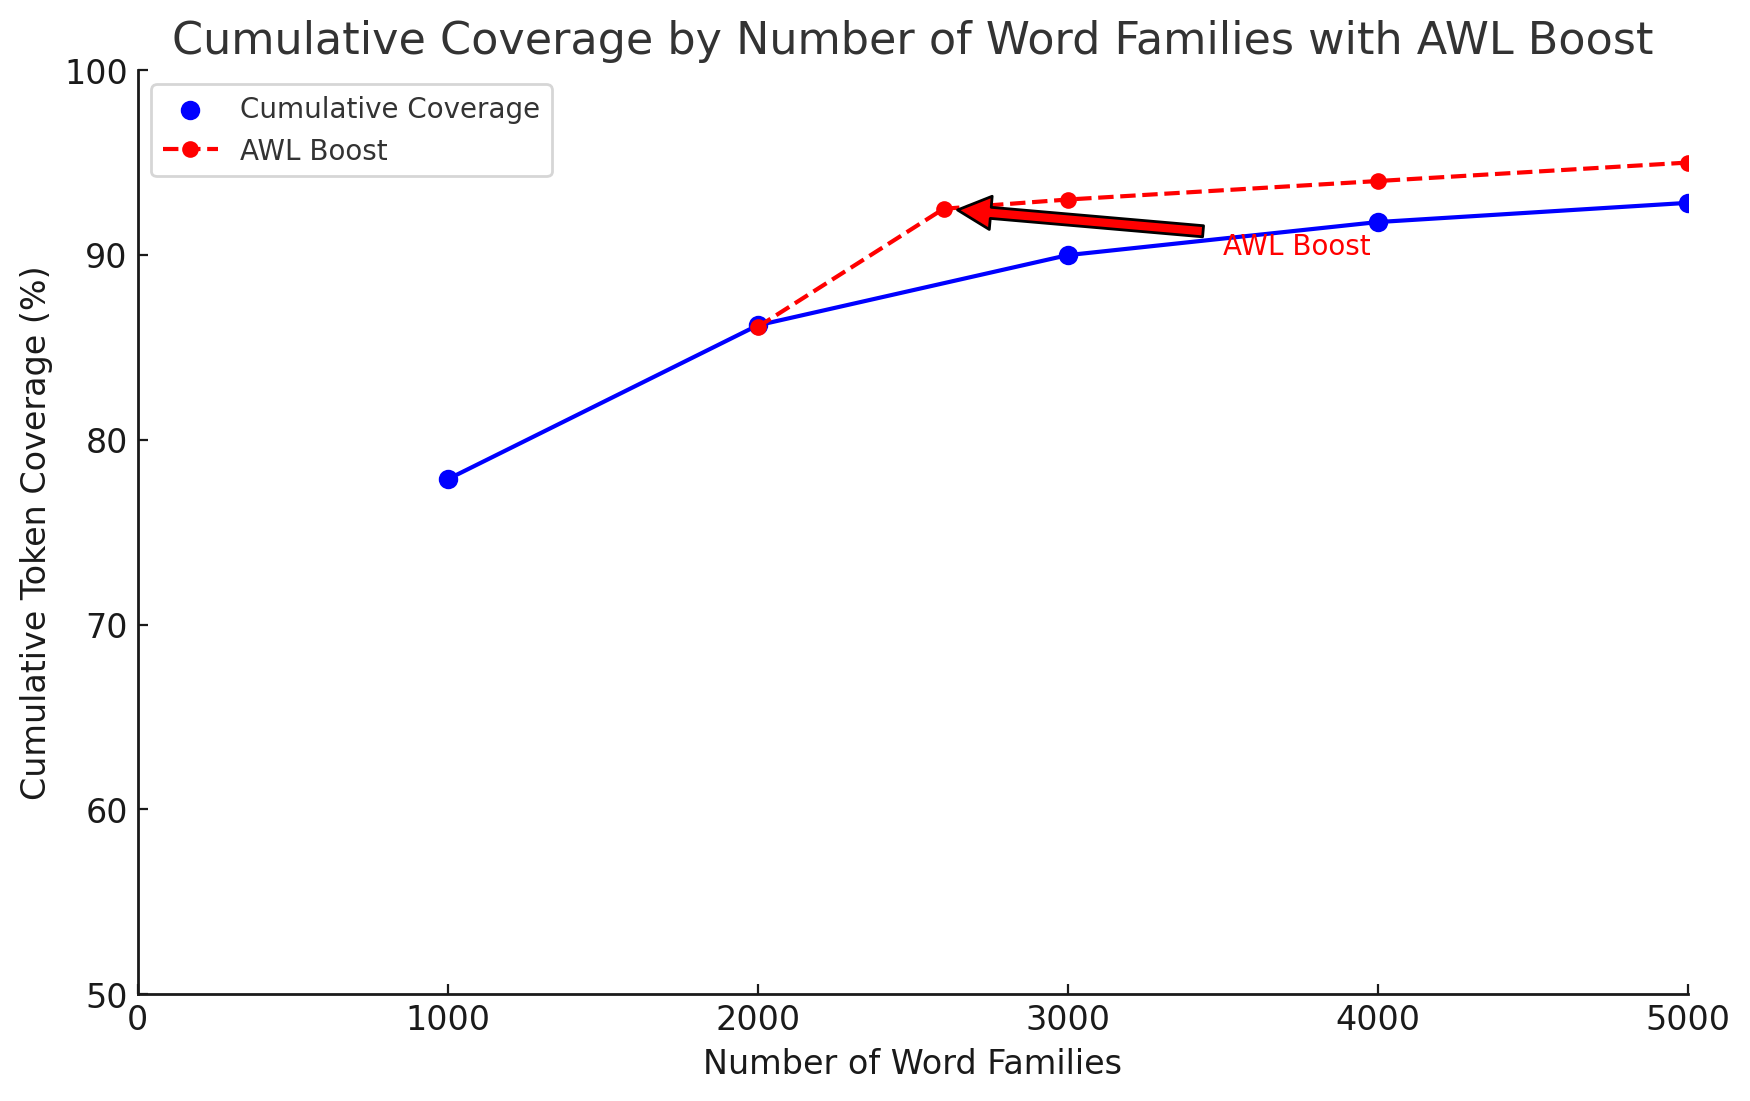
\includegraphics[width=0.8\linewidth]{figures/AWLboost.png}
    \caption{Cumulative token coverage of the LOB corpus by number of word families known, with a stylized illustration of the effect of studying the 570 words of the Academic Word List (AWL).}
    \label{fig:AWL boost}
\end{figure}

Now, think about \textit{humble} and \textit{potential} again. \textit{Humble} is about half way between 5,000 and 6,000 on the x axis. Look at how flat the curve is there. Each new word hardly adds any coverage of the text. But \textit{potential} is at about 1,000 on the x axis. There, the curve is still rising fast. Each new word makes a big difference. Each new word really counts.

Teach your learners words that count.

\begin{tcolorbox}[title=Exercise: Vocabulary Size and Coverage, colback=white, colframe=purple!75!black, fonttitle=\bfseries]
1. Approximately how many word families does a learner need to know to understand:
   \begin{enumerate}
      \item 80\% of a typical English text?
      \item 95\% of a typical English text?
      \item 98\% of a typical English text?
   \end{enumerate}

2. Why is 98\% coverage considered important for comfortable reading comprehension?

3. How might knowing about the Academic Word List (AWL) change your approach to teaching vocabulary to students preparing for university study?

4. Explain why learning the first 1,000 most frequent words in English is more beneficial than learning the next 1,000 most frequent words.
\end{tcolorbox}

\section{Selecting Vocabulary for Instruction} \label{sec:selecting-vocab}
\subsection*{The importance of word frequency}

Word frequency plays a crucial role in determining which words ``count'' most for learners. Corpus linguistics research demonstrates that a relatively small number of high-frequency words account for a large percentage of tokens in typical texts. For instance, the most frequent 1,000 word families in English cover approximately 80\% of written text \citep{Nation2013}.

This frequency distribution has significant implications for vocabulary pedagogy:

\begin{itemize}
    \item \textbf{Prioritization:} High-frequency words offer learners the greatest return on their learning investment. Table~\ref{tab:word-frequency} illustrates how dramatically word frequency drops off.
    
    \item \textbf{Text selection:} When choosing texts or designing activities, consider vocabulary load. Aim for materials where learners know 95-98\% of the words, allowing for comfortable reading and inference of unknown words from context.
    
    \item \textbf{Tiered approach:} Begin with the most frequent 1,000 words, then progress to subsequent frequency bands. This ensures learners build a solid foundation of useful vocabulary.
    
    \item \textbf{Caution with idioms and low-frequency words:} While these may hold intrinsic interest, they often offer limited utility for learners at lower proficiency levels. Any word, phrase, expression, or idiom that appears less frequently than 20 times per million words is considered a \textsc{low frequency item}, and teachers and students should carefully consider whether it's worth focusing on in class \citep{Nation2013}.
    
    \item \textbf{Unreliability of intuition:} Native speaker intuitions about word frequency often prove unreliable. Words that seem common to proficient speakers may not be high-frequency items. For example, \textit{humble} falls outside the top 3,000 most frequent words in English, despite its perceived commonality among native speakers.
\end{itemize}

\begin{table}[ht]
\centering
\caption{Word frequency drop-off}
\label{tab:word-frequency}
\begin{tabular}{lrr}
\textbf{Word family} & \textbf{Rank} & \textbf{Frequency per million words} \\
\textit{the} & 1 & 60,800 \\
\textit{you} & 10 & 12,800 \\
\textit{such} & 100 & 900 \\
\textit{purchase} & 1,000 & 90 \\
\textit{negotiate} & 2,000 & 35 \\
\end{tabular}
\end{table}

By integrating word frequency considerations with our understanding of vocabulary size and coverage, we can make more informed decisions about which words to prioritize in instruction. This approach ensures that learners acquire the most useful vocabulary efficiently, maximizing their ability to comprehend and communicate in English.

Figures \ref{fig:AWL boost} and \ref{fig:lemma-coverage} both illustrate the relationship between vocabulary size and text coverage, but they do so using slightly different metrics and data sources. This dual perspective helps us understand the general pattern while also highlighting some nuances in how we measure vocabulary knowledge.

%\begin{figure}
%    \centering
%    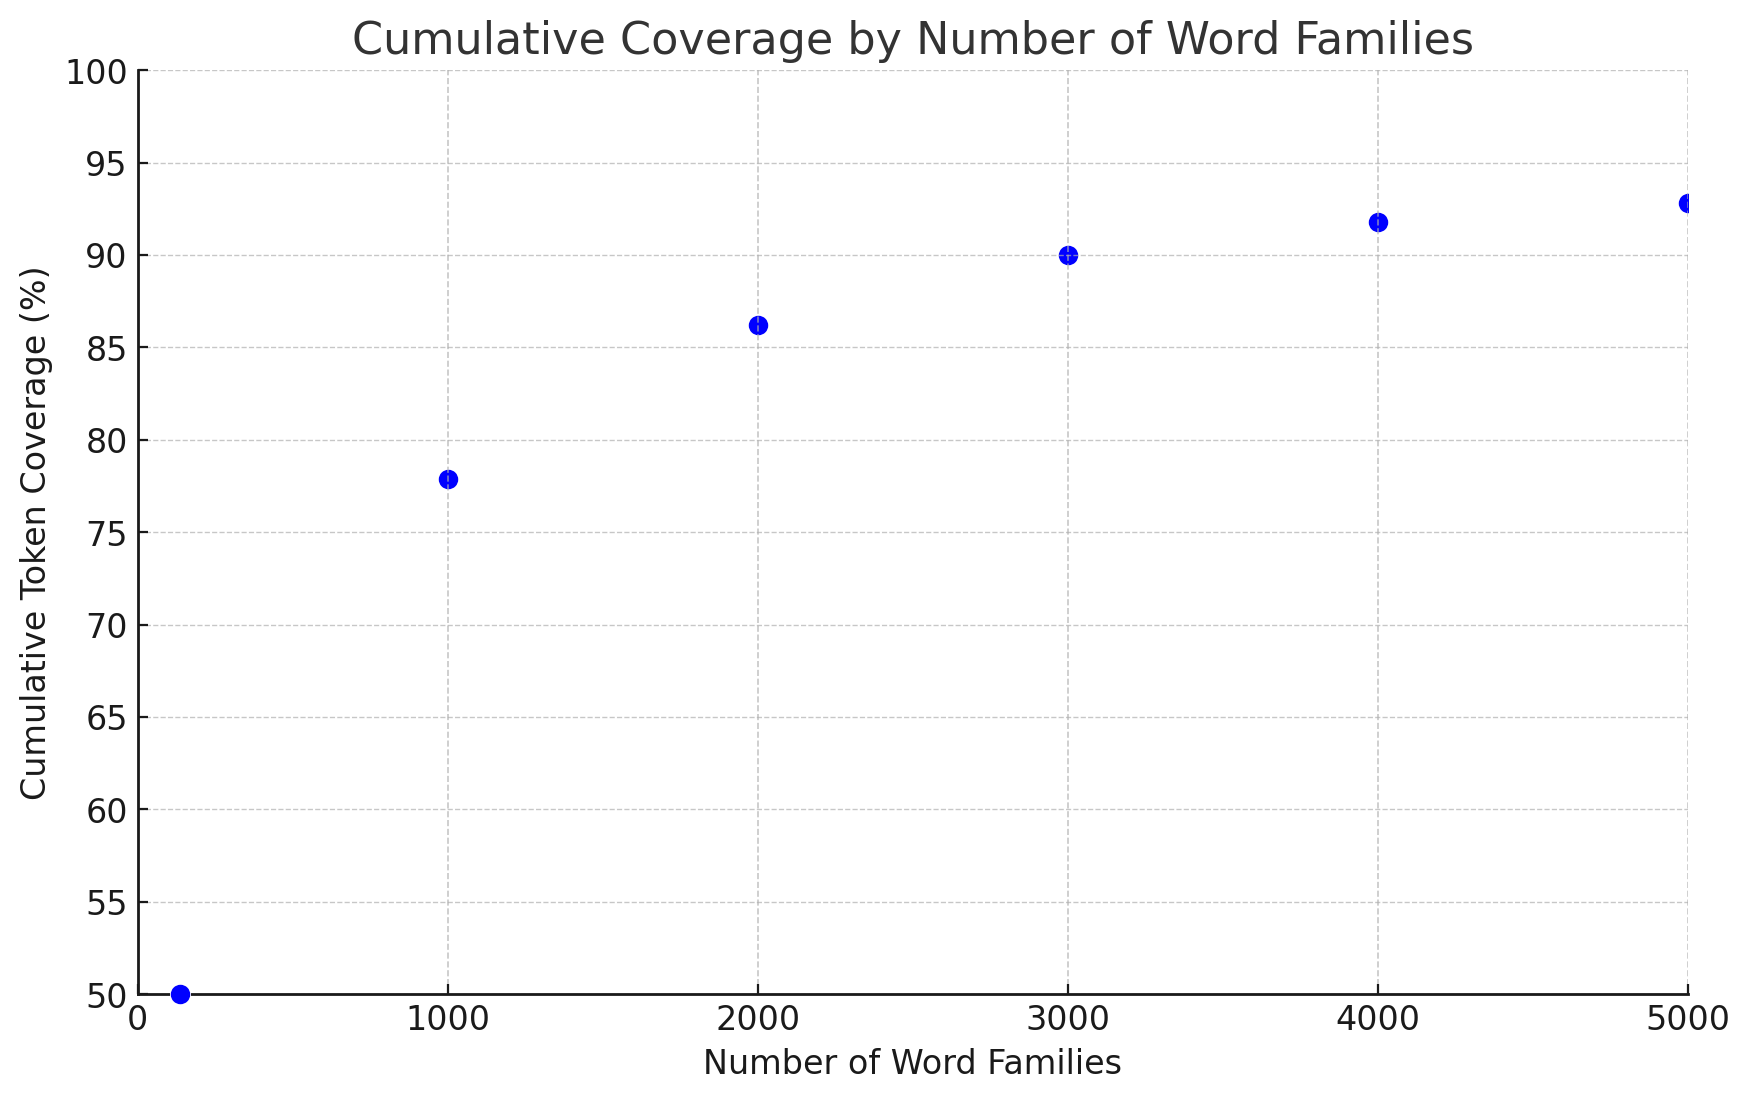
\includegraphics[width=0.8\linewidth]{figures/cumulative-families.png}
%    \caption{Cumulative lexical coverage of the LOB corpus as a function of number of word families known \citet[64]{nation_2006}.}
%    \label{fig:word-family-coverage}
%\end{figure}

\begin{figure}
    \centering
    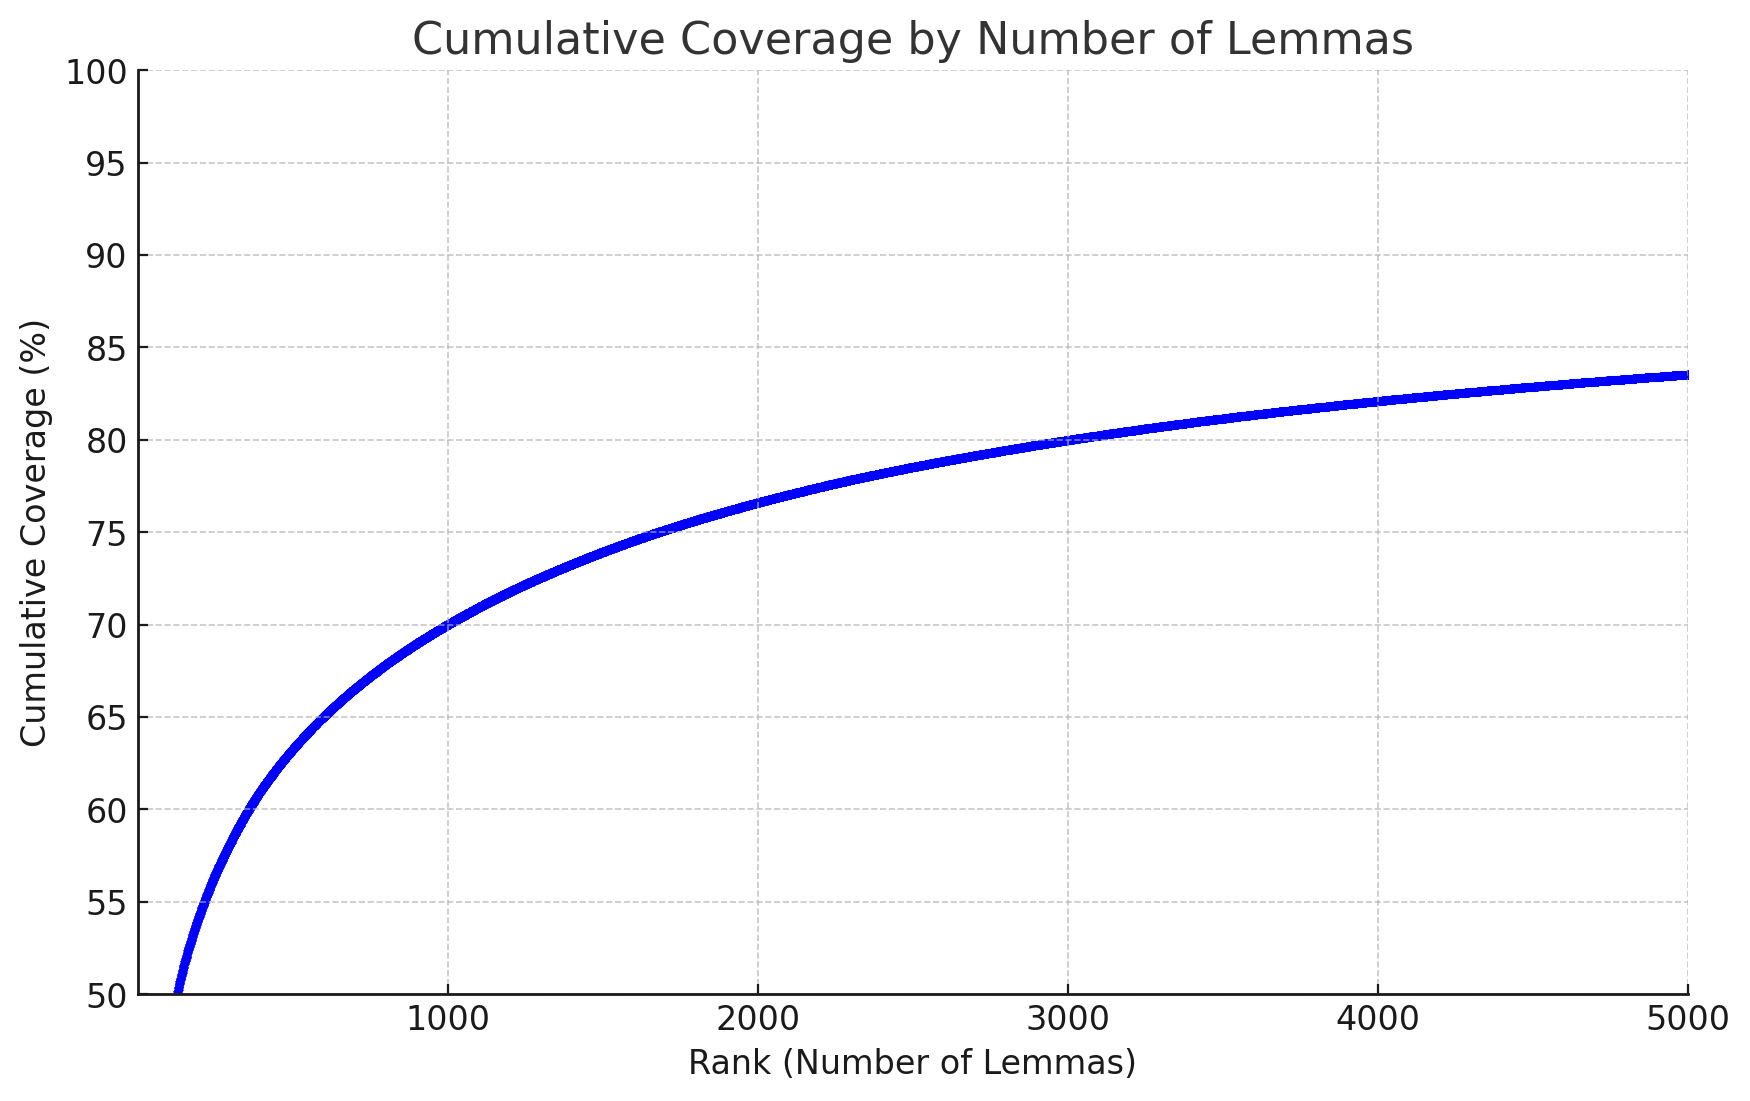
\includegraphics[width=0.8\linewidth]{figures/cumulative-lemmas.png}
    \caption{Cumulative lexical coverage of the COCA corpus as a function of number of lemmas known \citep{wordfrequency_info}.}
    \label{fig:lemma-coverage}
\end{figure}

The blue dots in Figure \ref{fig:AWL boost} show the cumulative coverage of the Lancaster-Oslo-Bergen Corpus as a function of the number of word families known. A word family includes not only inflections but also closely related derived forms (e.g., \textit{run}, \textit{runs}, \textit{ran}, \textit{running}, \textit{runner}, \textit{runners} would be one word family). This graph shows that knowledge of the 5,000 most frequent word families covers approximately 94\% of the tokens in its corpus.

In contrast, Figure \ref{fig:lemma-coverage} presents similar information but is based on the more recent and much larger Corpus of Contemporary American English (COCA) and uses lemmas. A lemma includes a base word and its inflected forms (e.g., \textit{run}, \textit{runs}, \textit{ran}, \textit{running} would be one lemma). This graph demonstrates that knowing the most frequent 5,000 lemmas provides coverage of about 84\% of the tokens in the corpus. This level appears lower than the word-family coverage simply because a word family often includes multiple lemmas.

While the specific numbers differ due to the different counting units and corpora used, both figures illustrate the same crucial point: there are diminishing returns as one learns more and more words. The steepest part of both curves is at the beginning, showing that learning the most frequent words (whether counted as lemmas or word families) provides the greatest boost in text coverage. As we move to less frequent vocabulary, each additional word learned contributes less to overall text coverage.

This pattern has important implications for vocabulary instruction. It suggests that focusing on the most frequent words~-- perhaps the top 2,000 to 3,000~-- will give learners the biggest ``bang for their buck'' in terms of improving their ability to understand texts. Beyond this point, the flattening of the curve indicates that learners need to acquire many more words for smaller gains in coverage.

It is important to note, though, that these graphs represent averages across a large corpus. The actual vocabulary needed can vary significantly depending on the specific genre or context. For instance, academic texts or specialized technical documents may require knowledge of less frequent but field-specific vocabulary that wouldn't be captured by these general corpus-based figures.

\subsubsection{What does this mean for comprehension?}
Research shows a strong correlation between a learner's vocabulary size and their level of comprehension \citep{Droop2003}. This connection underscores why expanding learners' vocabularies is a primary goal in language classes.

\citet{Schmitt2011} studied the comprehension level of 661 ``non-native speakers'' of English on two separate tests.\footnote{The \textit{N}=1,285 in Table 2 (p. 34) suggests that about 5\% of participants submitted only one test.} Their results are shown in Figure~\ref{fig:Schmitt2011}. As the figure shows, ``the results revealed a relatively linear relationship between the percentage of vocabulary known and the degree of reading comprehension'' \citep[26]{Schmitt2011}.

\begin{figure}
    \centering
    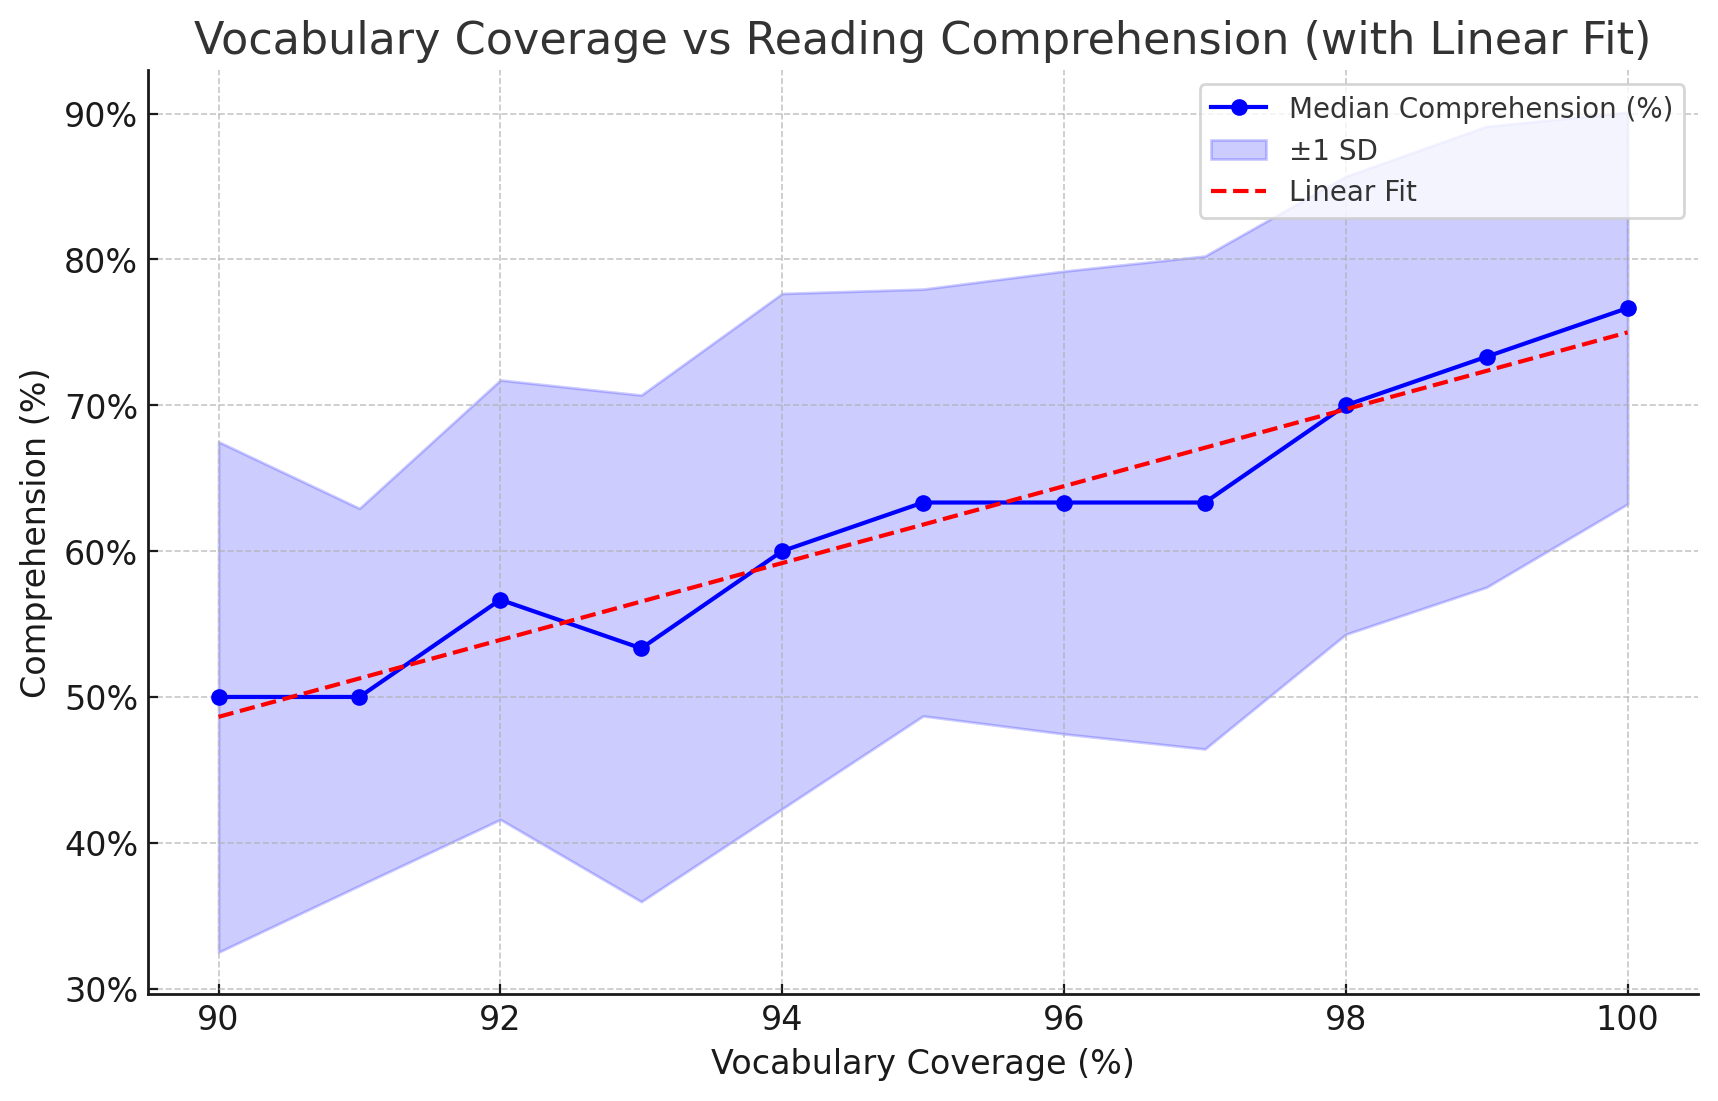
\includegraphics[width=0.8\linewidth]{figures/VocabCoverage.png}
    \caption{Vocabulary coverage vs. reading comprehension. The blue line shows median comprehension with ±1 SD shaded, and the red dashed line represents the linear fit, emphasizing the nearly linear relationship between vocabulary knowledge and comprehension \citep{Schmitt2011}.}
    \label{fig:Schmitt2011}
\end{figure}

The linear fit in the study suggests a strong relationship between vocabulary coverage and reading comprehension. For each 1\% increase in vocabulary coverage, comprehension improves by approximately 2.6 percentage points. It's important to note that the percentage known refers to the words in the reading passage, as tested in the study.

To understand the implications for lower vocabulary levels, we need to extrapolate from the available data. The lowest percentage of known words in the study was 90\%. Generally, it requires knowledge of about 3,000 words to achieve this level of coverage of a randomly chosen text. 

If we assume the relationship remains linear at lower levels, we can estimate that knowing 2,000 words would provide about 82.5\% coverage, corresponding to roughly 30.2\% comprehension. Similarly, a vocabulary of 1,000 words might yield approximately 77.9\% coverage and a mere 18\% comprehension level.

These projections highlight just how debilitating and inadequate knowing 80\% of the words in a text can be. At this level, comprehension is severely impaired, making effective reading impossible. 

Now, it's crucial to approach these extrapolations cautiously. The model's linear relationship may not hold up at very low vocabulary levels, and other factors could influence comprehension at these extremes. It might not be that bad. On the other hand, it might be even worse. Either way, it should help you to see how unfair it is to ask students who know 80\% of the words to guess the other 20\%.

\subsubsection{The Academic Word List}

Figure \ref{fig:AWL boost} illustrates the cumulative token coverage of English text as a function of the number of word families known, with an additional emphasis on the impact of learning Coxhead's (\citeyear{coxhead2000academic}) Academic Word List (AWL).

The blue solid line represents the general cumulative coverage achieved by knowing an increasing number of word families across various genres. It shows that knowing 1,000 word families provides about 78\% coverage, 2,000 word families reaches approximately 86\% coverage, and 5,000 word families covers about 93\% of tokens in typical texts.

The red dashed line demonstrates the ``AWL Boost'' - the additional coverage gained by learning the Academic Word List alongside the most frequent word families. It's crucial to note that this boost applies specifically to academic English texts, not to other genres such as novels, conversational English, or general non-academic writing.

This AWL boost is most pronounced around the 2,000--3,000 word family mark. At about 2,000 word families, the AWL provides a significant jump in coverage of academic texts, pushing it from about 86\% to nearly 93\%.

The graph effectively illustrates two key points:

\begin{enumerate}
    \item The principle of diminishing returns in vocabulary learning: The steepest gains in coverage occur in the first 2,000 word families, with the curve gradually flattening as more words are learned.
    \item The efficiency of learning the AWL for academic purposes: By focusing on these academically relevant words in addition to the most frequent 2,000-3,000 word families, learners can achieve a coverage level in academic texts that would otherwise require learning many more general vocabulary items.
\end{enumerate}

This visualization underscores the importance of strategic vocabulary learning, highlighting how targeted word lists like the AWL can significantly enhance text coverage in specific contexts, particularly for academic reading and writing.


\subsection*{The frequencies of individual words}\label{sec:word-frequency}

Most people are surprised at how quickly the frequencies of words drops off. Consider the following table.

\begin{tabular}{lrr}
\textbf{Word family} & \textbf{Rank} & \textbf{Frequency per million words} \\
\textit{the} & 1 & 60,800 \\
\textit{you} & 10 & 12,800 \\
\textit{such} & 100 & 900 \\
\textit{purchase} & 1,000 & 90 \\
\textit{negotiate} & 2,000 & 35 \\
\end{tabular}\\

Note that any word, phrase, expression, or idiom that appears less frequently than 20 times per million words is (for various practical and theoretical reasons) a \textsc{low frequency item}, and teachers and students should probably not waste class time focusing on it \citep[16]{Nation2013}.

Teach your learners words that count.

\subsubsection{Prioritizing Vocabulary: The Role of Opportunity Cost} \label{sec:opportunity-cost}

A crucial concept from economics that many English teachers overlook is \textsc{opportunity cost}. In the context of vocabulary instruction, opportunity cost refers to the potential benefit lost when choosing to teach one word over another. Every word taught is a word not taught. Every minute spent on low-frequency words is a minute not spent on high-frequency words. Every choice has its cost.

When teachers and learners select vocabulary targets, they are implicitly assigning value to those words, suggesting that these chosen words are more valuable than others not selected. One way to visualize this concept is to imagine a spectrum of words, with the words that learners are most likely to encounter frequently and find useful in their daily lives at one end and rarely-encountered or used words at the other.

Consider, for example, teaching the word \textit{humble}. A teacher might think, ``It could be useful someday,'' or ``students need this word to understand today's reading.'' True, but \textit{humble} appears only about 10 times per million words in the COCA, in about 1.6\% of the texts in the corpus. At number 5,725 on the list, it's well towards the ``rarely-encountered'' end of our word spectrum, far from the frequent and widely useful words that should be our priority.

Contrast that with, say, \textit{potential}, which is word 1,270, appearing roughly 115 times and occurring in about 10\% of the texts in the corpus. If your students know neither \textit{humble}, nor \textit{potential}, then choosing \textit{humble} incurs a significant opportunity cost.

Even if the students already know \textit{potential}, there are more than 4,400 other words on that spectrum after \textit{potential} with lower opportunity costs than \textit{humble}. Given that it's unrealistic to expect to teach even half of them, \textit{humble} shouldn't even be in contention.

Why might a word like \textit{humble} turn up in a lesson then? A common pitfall in vocabulary instruction is overvaluing immediate needs at the expense of long-term utility. We often prioritize words required to understand a specific sentence or text at hand. But if you had time to teach only one word, would you choose the one needed for today's lesson, or the one needed for a lifetime of communication? The most valuable words open doors daily; the least valuable, not even a door a year.



\subsubsection*{How many words do we know?}

For the same reasons expressed above, it's hard to say how many words students will know at each level. To this, we add the confounding factors of Spanish-speaking students, for instance, who come to English already knowing a lot of vocabulary from their L1 and Vietnamese students, for instance, whose L1 shares almost no vocabulary with English. Nevertheless, the following chart should give you some idea of how many words are known at various levels.

Figure \ref{fig:voc-size-est} shows estimates of the average number of word families known at various proficiency levels for English language learners and various Anglophone groups, including 20- and 60-year olds, and highly-educated adults.

\begin{figure}
    \centering
    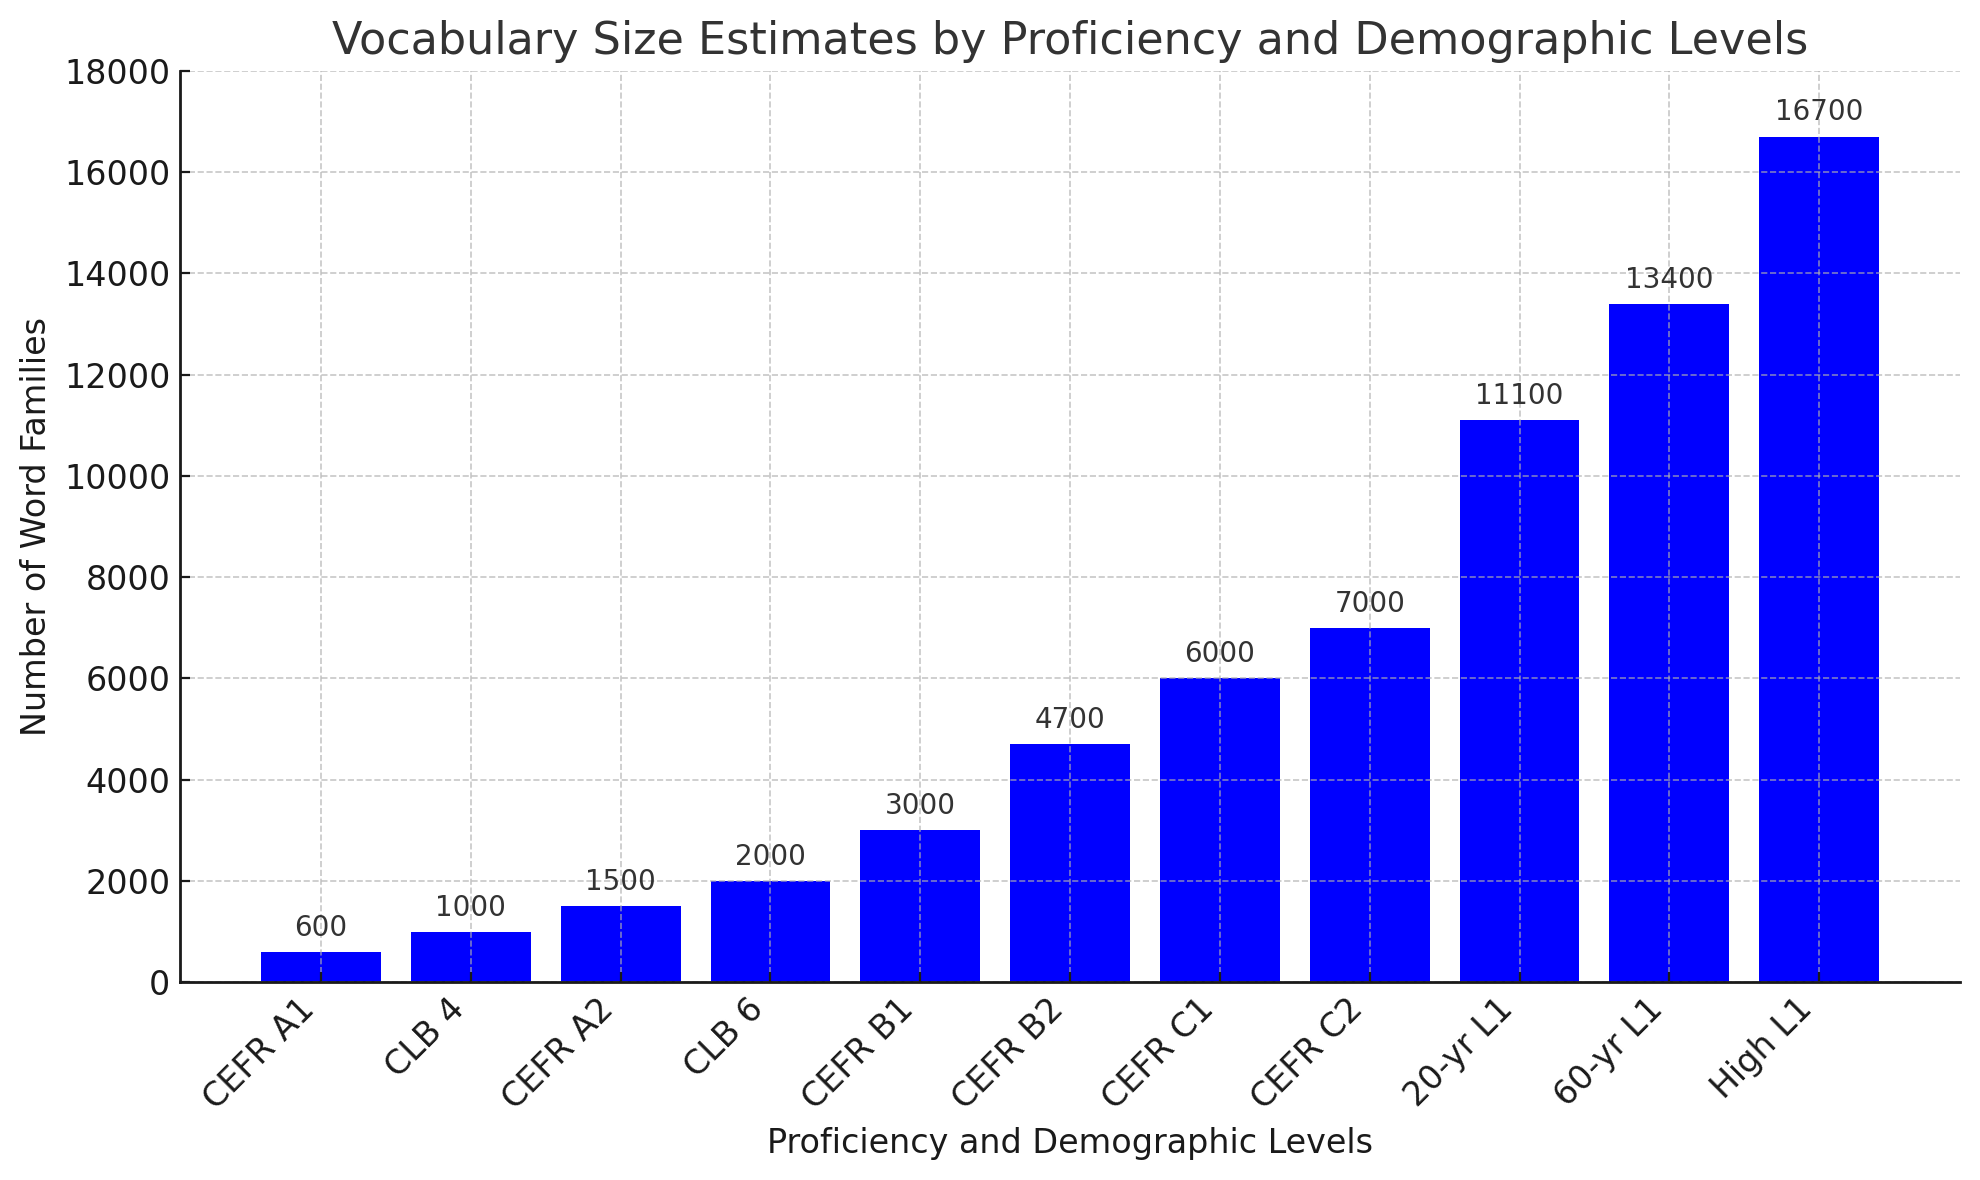
\includegraphics[width=0.8\linewidth]{figures/vocab-size-est.png}
    \caption{Vocabulary size estimates across proficiency and demographic levels based on cumulative word families \citep{brysbaert2016, capel2010, capel2012}.}
    \label{fig:voc-size-est}
\end{figure}


It's also hard to find a good test of your personal vocabulary size, but \href{https://www.vocabularytester.com/vocabulary-test}{this one}'s not bad. For students, \href{https://my.vocabularysize.com/}{my.vocabularysize.com} is a good test to provide an estimate of the number of word families that they know.

\subsubsection*{Vocabulary goals}

This understanding about coverage helps us set our learning goals. Once students know about 3,000 word families, they are more or less ready to deal with real-world texts on their own. This means that the vocabulary goal of our language classes is to get students to the 3,000-word level as quickly as possible. And, as the graphs show us, the most common words are much more common than the less common words. The first 1,000 words are of utmost importance. The next 1,000 words are also useful, but far less than the first thousand. The curve flattens quickly beyond this.

One consequence of this way of thinking is a careful focus on the most frequent words. We should, of course, not be wasting our students' time teaching them words like \textit{archipelago} and \textit{obsequious}, but even relatively ``common'' words like \textit{humble} fall outside of the top 3,000 word families that are worth teaching. It might seem obvious that we teach the most important things, but there are many words that appear in teaching materials and lesson plans that are not high-frequency words. In fact, it's incredibly common for teachers and textbook writers to spend~-- I'd say ``waste''~-- a lot of time on them.

\subsection{Grouping Vocabulary}

It might seem intuitive to teach semantically related words together~-- zoo animals, colour words, cooking verbs, adjectives of moods~-- but this approach can actually hinder learning in certain cases. Consider this example: 

You're learning a language called Verdic, and your teacher introduces these words:

\ea \textit{verd} `orange', \textit{vird} `lemon', \textit{vord} `grapefruit'
\z

\noindent The next day, you might remember the topic was citrus, but you'd likely struggle to recall what each word meant.

This illustrates a common problem with teaching semantic sets: While it facilitates remembering the general topic, the similar words often get mixed up, especially when they're phonologically or orthographically similar.

And yet, many textbooks take exactly this approach, introducing vocabulary in groups like ``means of transportation'' or ``months of the year''. Such groupings are generally counterproductive \citep{finkbeiner2003semantic, higa1963interference, schurgin2020psychophysical, waring1997negative}. It makes recalling the topic easier but matching words with specific meanings harder~-- and what we care about is the vocabulary, not the topic.

Another problem with this kind of grouping is it leads to the inclusion of low-frequency items to fill out the group. If you're doing colour words, \textit{red} is common, \textit{purple} is not.

And the problem doesn't apply just to semantic sets: alphabetical lists (e.g., \textit{comment},\textit{ commit},\textit{ committee},\textit{ common},\textit{ community},\textit{ company}) are equally bad.

Instead, consider these guidelines for grouping vocabulary:

\begin{itemize}
    \item Focus on words that aren't closely related: in meaning, spelling, or sound.
    \item Some general topical similarity is fine. For example, a ``going out for coffee'' theme could include words like \textit{table}, \textit{friend}, \textit{meet}, \textit{pay}, and \textit{a while}.
    \item Group words by frequency bands (e.g., top 500 word families, 501--1,000, 1,000--2,000, and Academic Word List). Be flexible around the edges of these bands, and avoid low-frequency words altogether.
    \item Teaching word families (e.g., \textit{bake}, \textit{baker}, \textit{bakery}) can be effective, as these are unlikely to be confused and provide repetition and variety.
\end{itemize}

Above all, ensure that your vocabulary selections are useful. Group them thematically and by frequency; teach word families but avoid words that are otherwise similar in meaning, spelling, or pronunciation.

\subsection{The problem with idioms}

Idioms present a particular challenge in vocabulary instruction, especially at lower proficiency levels. The primary issues stem from their low frequency and limited utility in everyday language use. Corpus studies indicate that even seemingly common idioms occur relatively infrequently in natural discourse. For instance, the idiom \textit{hit the jackpot} appears far less often than intuition might suggest \citep{reynolds2007idioms}.

The cultural specificity of many idioms further complicates their utility for language learners. Idiomatic expressions often rely on cultural knowledge or metaphors that may not translate across languages or cultures, potentially limiting their usefulness in international communication contexts. Moreover, the figurative nature of idioms can pose comprehension difficulties for learners, requiring additional cognitive processing to decode their non-literal meanings.

A common misconception among native speakers and some instructors is the overestimation of idioms' importance in everyday communication; though idioms as a class are common, individual idioms almost never are. This can lead to disproportionate emphasis on idiomatic expressions in language curricula, at the expense of more frequently occurring and broadly applicable vocabulary, incurring large opportunity costs (Section \ref{sec:opportunity-cost}).

Given these considerations, a more effective approach, particularly at lower proficiency levels, involves prioritizing high-frequency vocabulary and collocations. Teaching strategies for dealing with unfamiliar figurative language often proves more valuable than memorizing specific idiomatic expressions. As learners progress to higher proficiency levels, a very few common idiomatic expressions can be introduced gradually, focusing on those with higher frequency or particular relevance to learners' specific needs.

When idioms are incorporated into instruction, it is essential to provide clear context, explain their meanings and usage patterns, and offer opportunities for practice in appropriate situations. This approach ensures learners develop a balanced and useful vocabulary while gaining exposure to the idiomatic aspects of English, without overemphasizing low-frequency expressions.

\begin{tcolorbox}[title=Exercise: Word Frequency and Vocabulary Selection, colback=white, colframe=red!75!black, fonttitle=\bfseries]
1. Using your knowledge or intuition about word frequency, rank the following words families from most frequent (1) to least frequent (5):

\begin{enumerate}
    \item \textit{humble}
    \item \textit{the}
    \item \textit{potential}
    \item \textit{dolphin}
    \item \textit{negotiate}
\end{enumerate}

2. Now check the shape frequency in the COCA.

3. Now check the lemma frequency.

4. Explain why teaching \textit{humble} might have a higher opportunity cost than teaching \textit{potential}.

3. If you had to choose between teaching the words \textit{archipelago} and \textit{necessary} to intermediate English learners, which would you choose and why?

4. How might understanding word frequency affect your approach to vocabulary instruction? Give two specific examples.
\end{tcolorbox}

\section{Teaching and learning vocabulary} \label{sec:teaching-learning-vocab}
Vocabulary acquisition hinges on four key elements: 1) repetition of 2) useful words, with 3) variety in presentation and practice and 4) focused attention. 

The first pillar is repetition. Research indicates that effective learning usually requires multiple encounters with a word, optimally spaced over time. This principle aligns with the concept of spaced repetition, a technique proven to enhance long-term retention.

In selecting vocabulary for instruction, prioritize useful words. These typically encompass the most frequent 2,000 words in English, supplemented by an additional 1,000 words relevant to the learner's specific needs or field of study. For academic contexts, this might include terms from the Academic Word List.

Variety in presentation and practice is crucial. Effective vocabulary instruction exposes learners to words through multiple modalities: visual, auditory, and kinesthetic.\footnote{This has nothing to do with ``learning styles'', a theory which has been thoroughly debunked and is considered possibly detrimental by the \citet{apa2019learning}. Instead, it's supported by the dual-coding hypothesis \citep{ginns2005} we met in Section~\ref{sec:why-trees}.} This approach includes encountering words in diverse contexts, connecting them to images, and using them in various grammatical forms. Such variety fosters a robust network of associations, facilitating recall and use.

Attention forms the fourth pillar of vocabulary acquisition. Mere exposure to a word is insufficient; the depth of processing directly correlates with retention. The more a learner engages with a word's meaning, usage, and connotations, the higher the likelihood of long-term retention.

\begin{figure}
    \centering
    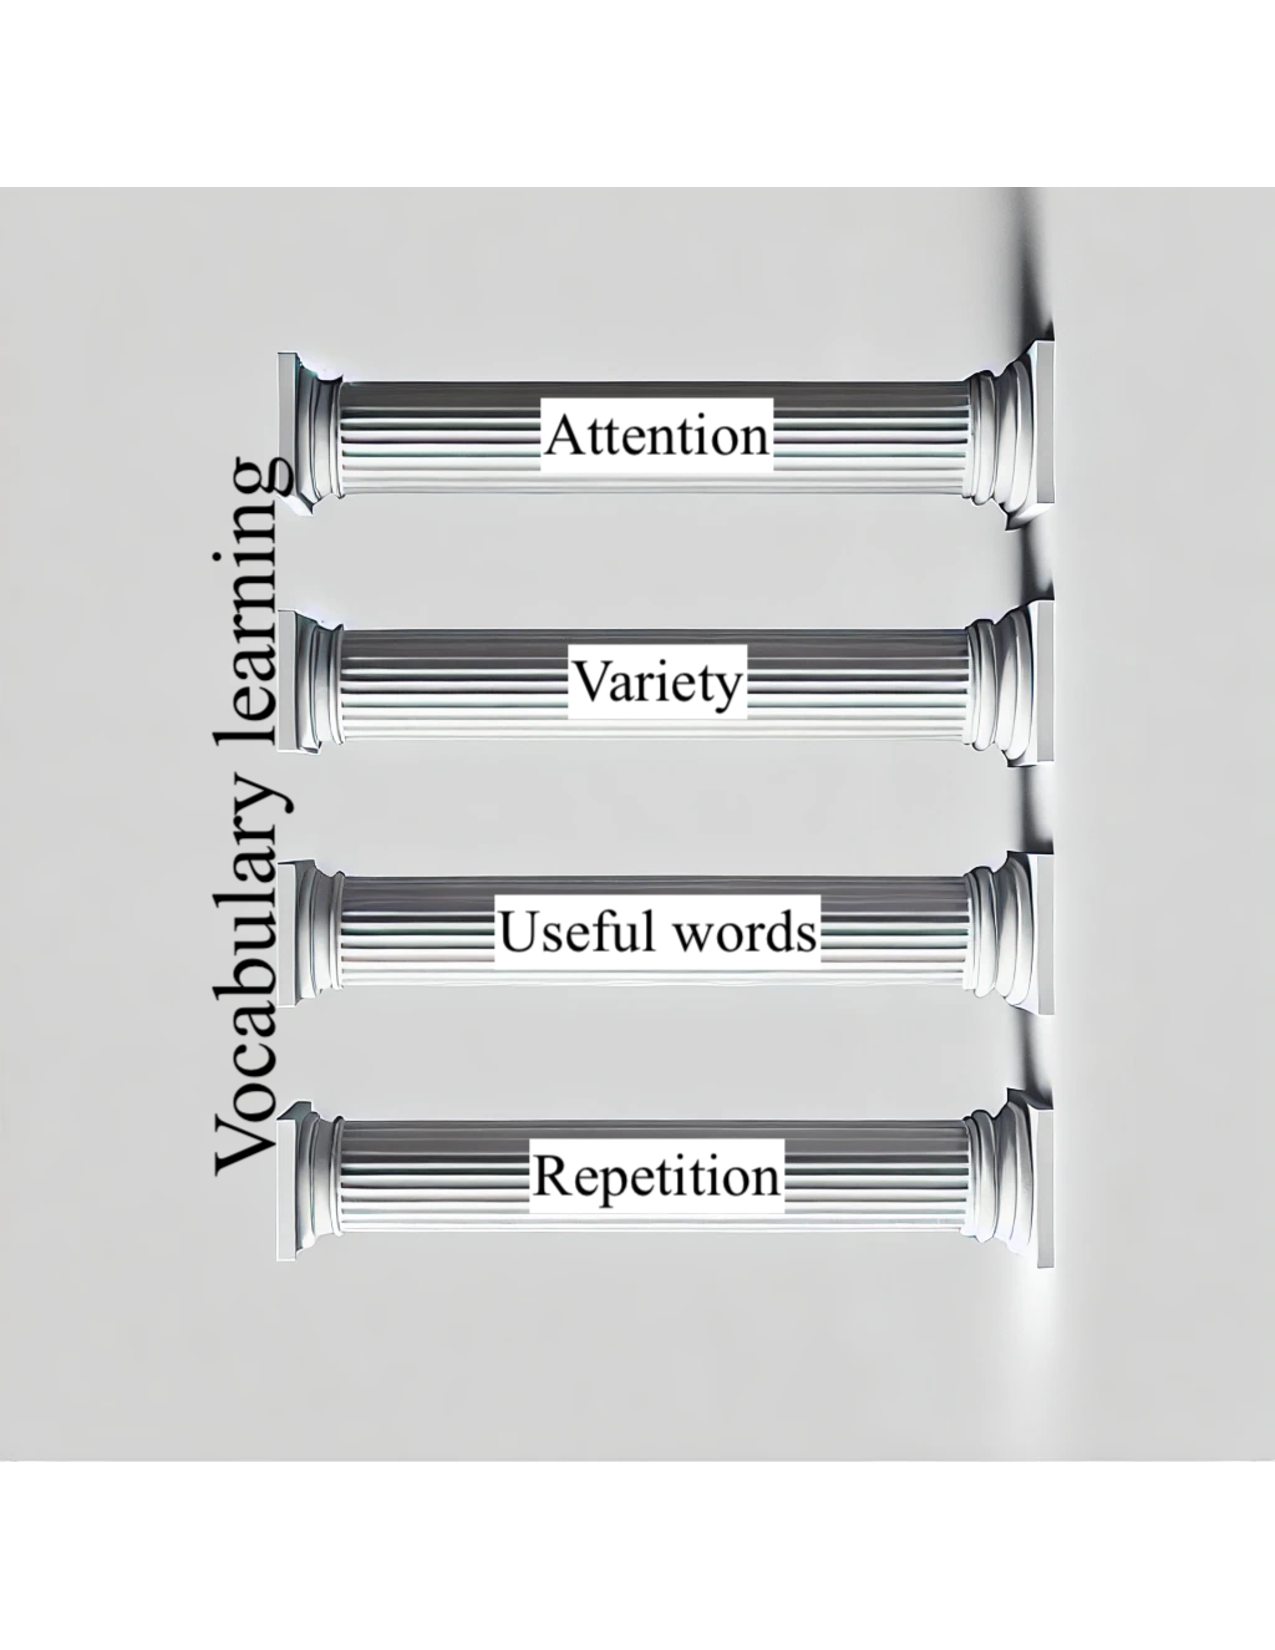
\includegraphics[width=0.5\linewidth]{figures/vocabPillars.pdf}
    \caption{The vocabulary-learning pillars.}
    \label{fig:vocab-pillars-AI}
\end{figure}

However, several barriers impede effective vocabulary learning. Motivation often presents the primary obstacle, particularly for activities like flashcard drilling, which many learners find tedious. And although there are many studies showing that students enjoy extensive reading \citep{Robb2013ER}, it's not a popular or common way to learn vocabulary. Time constraints pose another significant challenge, especially for adult learners balancing language study with other responsibilities.

\subsection{Explaining the Meaning of Words}\label{sec:explaining-words}

Explaining word meanings is a core skill for language teachers. While semantics deals with meaning in linguistics and philosophy, and lexicography focuses on dictionary definitions, we're concerned with practical techniques for the classroom.

When explaining word meanings, it's useful to keep our three pillars of vocabulary acquisition in mind. Repetition can be incorporated by revisiting explanations or using the new word in multiple contexts. Variety can be achieved through different explanation techniques, such as translation, definition, and visual aids. Attention is naturally engaged when students actively process new word meanings.

\subsubsection{Translation}

The easiest and most efficient way to explain a word's meaning is often to translate it. While some teachers shy away from using the L1, it's well justified both empirically and philosophically. It's true that L1 translations rarely capture a word's full meaning perfectly, but no other explanation method does any better. Translation is particularly useful for dealing quickly with low-frequency items that would otherwise consume too much class time.

\subsubsection{Other Techniques}

When translation isn't an option, consider these approaches:

\begin{itemize}
    \item Use brief, clear definitions focusing on core meanings or prototypical cases. For example, in explaining \textit{head}, keep in mind that all the various senses, including the part of the body and the company leader, revolve around the core meaning of `the top or front part of something'.
    \item For lower-level students, explain the meaning rather than paraphrasing. For example, compare these ways to convey the meaning of \textit{probably}.
    \begin{itemize}
        \item \textbf{Explanation:} If something is \textit{probably} true, or will \textit{probably} happen, there's a high chance of it.
        \item \textbf{Paraphrase:} having a high chance of being true
    \end{itemize}
    \item Use objects, pictures, gestures, or any other available resources.
\end{itemize}

\subsubsection{Improving Your Explanations}

Nobody's naturally good at explaining word meanings, but it's a crucial skill for language teachers. Improving requires deliberate practice. Here's a suggested routine:

\begin{enumerate}
    \item Choose a high-frequency or Academic-Word-List word
    \item Try to explain it
    \item Check a good dictionary like the \textit{Longman Dictionary of Contemporary English} (LDOCE)
    \item Revise your explanation
    \item Repeat steps 1--4 three times
    \item Wait until the next day and repeat the process once more
    \item Continue until you rarely need to revise (this may take hundreds of repetitions)
\end{enumerate}

Remember, if you expect your students to engage in deliberate practice (and you should), then you ought to be willing to do deliberate practice yourself. One way to practice is by contributing definitions to resources like the \textit{Simple English Wiktionary}.


\begin{tcolorbox}[title=Exercise: Explaining Word Meanings, colback=white, colframe=green!75!black, fonttitle=\bfseries]
1. Practice explaining the following words without using a dictionary. Then, compare your explanations with those in a learner's dictionary like the Longman Dictionary of Contemporary English:

\begin{enumerate}
   \item \textit{curious}
   \item \textit{despite}
   \item \textit{efficient}
   \item \textit{hesitate}
   \item \textit{impact}
\end{enumerate}

2. For each word above, identify whether it's likely to be a high-frequency or low-frequency word. Justify your answer.

3. Choose one of the words above and demonstrate how you would explain it using:
   \begin{enumerate}
      \item A brief definition
      \item An example sentence
      \item A visual aid or gesture (describe what you would draw or do)
   \end{enumerate}

4. Why might translation be an efficient method for explaining word meanings? What are some potential drawbacks?
\end{tcolorbox}

\newpage
\subsection{Vocabulary learning techniques}

Several effective techniques can enhance vocabulary acquisition. Each method incorporates at least one of the three pillars of vocabulary learning: repetition, variety, and attention. The most effective approaches will often engage all three pillars:

\paragraph*{Self-testing with spaced repetition (``flashcard drill'')} This technique is by far the most efficient and easiest way to learn a form-meaning pairing. In fact, a recent meta-analysis shows that the average person can learn a word a minute using this technique, and that's on a delayed post-test \citep{webb2020}. But it tends to be perceived as boring and requires significant consistent motivation, which most of us find unpleasant \citep{David2024}.

\begin{tcolorbox}[title=Flashcard Study Technique, colback=white, colframe=blue!75!black, fonttitle=\bfseries]

\textbf{Steps:}

\begin{enumerate}
    \item Put the L1 on one side of a word card and the target language (L2) on the other side.\footnote{L2 is often glossed as ``second language'', but, here, I mean it simply to be the language you intend to learn, whether it be your second or your twelfth.} (Or do the equivalent in some software).
    
    \item Set a goal for new words and review words.\\
    (At 15 new words per day, you can learn more than 5,000 form-meaning pairings in a year.)
    
    \item Place the new vocabulary first. Review vocabulary comes later.
    
    \item Decide if you're studying for production or reception. (We'll assume production.)
    
    \item Start studying. Continue until you've reached your goal.
    \begin{enumerate}
        \item Look at the first card in your L1 (L2 for receptive learning).
        \item Try to think what is on the other side. If possible, say it aloud.
        \item Check the other side.
        \item Note any discrepancies. (very important!)
        \item Judge your success.
        \item Replace the card in the pack based on success\\
        (Complete failure goes two cards from the front. Easy success goes right at the back.)
    \end{enumerate}
\end{enumerate}

\end{tcolorbox}
\newpage
\paragraph*{The keyword technique} This technique involves associating a new word with a similar-sounding word in the learner's native language, then creating a vivid mental image connecting the two. For example, to learn the Indonesian word \textit{parit} (meaning ``ditch''), an English speaker might use \textit{parrot} as a keyword and imagine a parrot digging a ditch. While effective, it can be challenging to implement consistently.

\begin{tcolorbox}[title=Keyword Technique Examples, colback=white, colframe=blue!75!black, fonttitle=\bfseries]

To illustrate the keyword technique, consider these examples:

\begin{wrapfigure}{r}{0.4\linewidth}

\includegraphics[width=0.5\linewidth]{figures/parrot.jpg}
\end{wrapfigure}
%Credit: Image created with ChatGPT 4o

\textbf{Example 1: Indonesian}


\begin{wrapfigure}{r}{0.5\linewidth}

\includegraphics[width=0.5\linewidth]{figures/relish.jpg}
\end{wrapfigure}
%Credit: Image created with ChatGPT 4o

\begin{itemize}
    \item Target word: \textit{parit} (meaning `ditch')
    \item Keyword: \textit{parrot}
    \item Mental image: A parrot digging a ditch
    \begin{itemize}
        \item A parrot performing a headstand in a ditch
        \item A parrot lying in a ditch, surrounded by scattered feathers 
    \end{itemize}
\end{itemize}



\textbf{Example 2: Japanese}
\begin{itemize}
    \item Target word: 嬉しい (\textit{ureshii}, meaning `happy')
    \item Keyword: \textit{relish}
    \item Mental image: A joyful jar of relish
    \begin{itemize}
        \item An ecstatic individual eating relish
        \item Someone gleefully swimming in relish 
    \end{itemize}
\end{itemize}

Memory is thought to be stickiest when students create personally meaningful and memorable associations. On the other hand, AI image generation is certainly much faster, and may be quite good.
\end{tcolorbox}
\newpage
\paragraph*{Guessing from context} This is a valuable skill for learners. Teachers should provide practice materials where learners know almost all the other words, replacing target words with non-words. Learners should be required to justify their guesses, analyzing syntactic categories and contextual clues. This is a commonly taught skill, but quite often it's assigned with texts which are too difficult. In order to be able to guess successfully, learners need to already know more than 98\% of the vocabulary.

\paragraph*{Classroom activities} Teacher-led classroom activities should encourage attention, recycling, retrieval from memory, and generation. Examples include cloze reviews, retelling stories, dictation, delayed copying, peer teaching with flashcard exchange, and vocabulary discussions.

\paragraph*{Extensive reading} Extensive reading involves reading a large volume of self-selected, easy, interesting texts. Some programs set a goal of 1 million words a year. The approach provides repeated exposure to vocabulary in varied contexts, improving overall language proficiency and attitudes to reading and learning.

\subsubsection{Deliberate practice}\label{sec:delib}

Deliberate practice, a concept central to skill acquisition, has significant implications for vocabulary learning. This approach involves focused, purposeful practice with specific goals, immediate feedback, and opportunities for repetition and refinement. In the context of vocabulary acquisition, deliberate practice encompasses several key elements.

Firstly, it requires setting specific, measurable learning objectives. For vocabulary, this might involve targeting a certain number of new words per week or achieving mastery of a particular semantic field. These goals should be challenging yet attainable, pushing learners beyond their current competence level.

Secondly, deliberate practice necessitates immediate, informative feedback. In vocabulary learning, this feedback might come from self-checking mechanisms, peer review, or instructor input. The immediacy of feedback allows learners to quickly identify and correct errors, reinforcing accurate knowledge and use of new words.

Thirdly, deliberate practice involves repetition and refinement. For vocabulary, this means encountering and using new words multiple times in varied contexts. Spaced repetition systems, whether digital or analog, can facilitate this process by systematically reintroducing words at optimal intervals for retention.

Deliberate practice is particularly well-suited to vocabulary learning. Vocabulary often comprises discrete units (individual words or phrases) that can be practiced in isolation, allowing for focused attention on specific items. Progress in vocabulary acquisition is relatively easy to measure and quantify, facilitating goal-setting and progress tracking. Moreover, vocabulary practice can be readily tailored to individual needs and proficiency levels.

To implement deliberate practice in vocabulary instruction, educators can employ several strategies:

\begin{enumerate}
    \item Provide clear, achievable goals for vocabulary acquisition, such as mastering a specific number of words from a frequency list.
    
    \item Offer regular, structured opportunities for word practice and review, incorporating both receptive and productive skills.
    
    \item Integrate immediate feedback mechanisms into vocabulary activities, allowing learners to quickly assess understanding and use of new words.
    
    \item Encourage learners to track their progress and set personal vocabulary goals, fostering autonomy and motivation.
    
    \item Use spaced repetition techniques to ensure optimal review intervals for newly learned words.
    
    \item Incorporate newly learned vocabulary into various contexts and tasks, promoting deeper processing and more robust retention.
\end{enumerate}

Deliberate practice naturally incorporates our three pillars of vocabulary acquisition. The repetitive nature of practice ensures multiple encounters with target vocabulary. Variety is achieved through diverse contexts and applications of the words being learned. The focused, goal-oriented nature of deliberate practice demands sustained attention. By consciously applying these principles, learners can maximize the effectiveness of their vocabulary study sessions.

By incorporating principles of deliberate practice, instructors can enhance the efficiency and effectiveness of vocabulary instruction. This approach not only accelerates vocabulary acquisition but also equips learners with strategies for continued, self-directed learning beyond the classroom.

It is important to note, though, that while deliberate practice is highly effective, it's cognitively demanding and is often experienced as tedious and monotonous. Students who can dedicate themselves to this kind of study will see large gains, but most can/do not. Instructors should balance this intensive approach with more incidental learning opportunities, such as extensive reading or communicative tasks, to maintain learner motivation and provide varied exposure to target vocabulary.


%\subsection{Incorporating word frequency in vocabulary instruction}

%Understanding word frequency can significantly enhance vocabulary instruction. Here are some specific strategies for integrating frequency-based approaches into your teaching:

%\begin{enumerate}
    %\item \textbf{Prioritize high-frequency words:} Focus the majority of your explicit vocabulary instruction on the most frequent word families. These words provide the greatest return on investment for learners, dramatically improving their ability to understand and produce English. For words beyond the top two or three thousand, rely on contextual learning.
    
    %\item \textbf{Use graded readers:} Select texts that are specifically written to include only the most frequent words at various levels. This allows students to practice extensive reading with texts that match their current vocabulary knowledge. (See \ref{sec:reading-fluency}.)
    
    %\item \textbf{Create frequency-based word lists:} Develop custom vocabulary lists for your students based on frequency data and their specific needs. Tools like the \href{https://www.wordandphrase.info/frequencyList.asp}{COCA frequency list} can help you identify high-frequency words relevant to your students' goals.
    
    %\item \textbf{Teach word families:} When introducing a new high-frequency word, teach its common derivations as a set. For example, when teaching \textit{create}, it may be useful to mention \textit{creates}, \textit{created}, \textit{creating}, \textit{creation}, and \textit{creative}. This approach maximizes the utility of each word learned.
    
    %\item \textbf{Use corpus tools in class:} Introduce students to corpus tools like COCA (\url{https://www.english-corpora.org/coca/}) to explore word frequency and usage. This can help develop their metacognitive awareness of vocabulary learning strategies.
    
    %\item \textbf{Teach high-frequency academic words:} For students preparing for academic study, focus on words from the Academic Word List (AWL) after they have mastered the most frequent 2,000 general words.
    
    %\item \textbf{Address misleading intuitions:} Explicitly discuss with students (and possibly colleagues) how native speaker intuitions about word frequency can be misleading. This can help justify your focus on certain words that might seem ``too simple'' to advanced learners.
    
    %\item \textbf{Frequency-informed extensive reading:} Encourage extensive reading of texts slightly above students' current level. Aim for texts where students know about 98\% of the words, allowing them to read with comfort.
    
    %\item \textbf{Caution with idioms and low-frequency words:} Be extremely selective when teaching idioms and low-frequency words. While these can be interesting, they often offer limited utility, especially at lower proficiency levels. When you do teach them, explicitly note their relative rarity to set appropriate expectations for usage.
%\end{enumerate}

%As you implement these frequency-based strategies, keep in mind the three pillars of vocabulary acquisition. Repetition is naturally built into the focus on high-frequency words, as learners will encounter these words often. Variety can be achieved by presenting these words in diverse contexts and through multiple activities. Attention is engaged when learners actively work with frequency data and make conscious choices about which words to prioritize. By aligning our frequency-based approach with these fundamental principles, we can create a robust and effective vocabulary instruction program.

\begin{tcolorbox}[title=Warning: Mindless Repetition, colback=white, colframe=red!75!black, fonttitle=\bfseries]
It's crucial to distinguish deliberate practice from mindless repetition. Simply reciting words or flipping through flashcards without engaging with their meaning is a colossal waste of time. Effective vocabulary learning demands active, focused attention that encourages deeper processing and meaningful connections. If you catch yourself or your students merely going through the motions, stop and switch to a more engaging activity. Remember: it's not about how many times you repeat a word, but how often you repeat it with attention.
\end{tcolorbox}

\begin{tcolorbox}[title=Exercise: Teaching and Learning Vocabulary, colback=white, colframe=orange!75!black, fonttitle=\bfseries]
1. Describe the three pillars of effective vocabulary acquisition and give an example of how each might be applied in a classroom setting.

2. Why might teaching words in semantic sets (e.g., all the colours at once) be less effective than other grouping strategies?

3. Create a keyword technique example for teaching the word "melancholy" to English language learners.

4. Explain why extensive reading can be an effective method for vocabulary acquisition. What conditions need to be met for it to be most effective?

5. Design a short activity that incorporates spaced repetition for teaching vocabulary.
\end{tcolorbox}

\subsection{A note on collocations}\label{sec:collocations}

While individual words form the basic units of vocabulary, words often occur in predictable combinations called \textsc{collocations}. For example, in Canada, we make a decision but take a break (not \textit{take a decision} or \textit{make a break}). We say \textit{heavy}~-- not \textit{strong}~-- \textit{rain} but \textit{strong}~-- not \textit{heavy}~-- \textit{wide}. Competent speakers generally recognize and use these combinations, but they can pose challenges for language learners.

Given their importance for natural-sounding production, it might seem logical to teach collocations explicitly. I would advise against that \citep{reynolds2019against}.

\begin{itemize}
    \item Most collocations are relatively infrequent. Even common words like \textit{decision} have multiple collocations (\textit{make}, \textit{reach}, \textit{arrive at}, etc.), each appearing far less frequently than the base word.
    
    \item The number of possible collocations is vast. Even focusing on ``common'' collocations would require learning thousands of combinations.
    
    \item Many collocations are somewhat predictable from the meaning of their parts. For instance, once you know that \textit{heavy} means `having great weight or force', combinations like \textit{heavy rain}, \textit{heavy traffic}, and \textit{heavy workload} become more intuitive.
\end{itemize}

Given these considerations, along with our earlier discussion of opportunity cost (\ref{sec:opportunity-cost}), explicit collocation instruction rarely justifies the time investment. Instead, learners typically acquire collocations naturally through extensive exposure to the language, particularly through reading and listening.

This doesn't mean ignoring collocations entirely. When teaching a new word or giving examples, including one or two of its most frequent collocations can be helpful. For instance, when introducing \textit{decision}, noting that it commonly occurs with \textit{make} takes just a few seconds and provides useful context. But dedicated collocation exercises or extensive collocation lists typically offer poor return on investment compared to other vocabulary learning activities.

\ea 
\ea Time spent learning that we say \textit{heavy rain} rather than \textit{strong rain} might be better spent learning another high-frequency word.
\ex Most collocations will be acquired naturally through exposure to the language in meaningful contexts.
\z
\z

This approach to collocations aligns with the broader principles of vocabulary instruction: prioritize high-frequency items, consider opportunity costs, and favour efficient learning strategies over comprehensive but time-consuming approaches.

\section{Summary}

This chapter explored various aspects of vocabulary, from its basic components to effective teaching and learning strategies. Here's a recap of the main points:

\subsection*{Word Construction and Definition}

\begin{itemize}
\item Morphology: Words are formed from bases and affixes
\item ``Word'' can mean different things: semantic units, syntactic units, families, lemmas, or tokens
\item These distinctions matter for setting learning goals and selecting materials with good text coverage
\end{itemize}

\subsection*{Vocabulary Size and Coverage}

\begin{itemize}
\item Students need to know about 98\% of words in a text for comfortable reading
\item That's about 8,000-9,000 word families for general English
\item But 2,000 word families cover about 80\% of most texts
\end{itemize}

\subsection*{Word Frequency and Selection}

\begin{itemize}

\item Teach key affixes; most aren't worth focused attention
\item Word frequency drops off dramatically after the most common words
\item The top 1,000 word families are vastly more frequent than the next 1,000
\item Focus on high-frequency, useful words for the biggest impact
\item Consider the opportunity cost of teaching low-frequency words
\item Be cautious with idioms~-- they're rarely as useful as they seem
\end{itemize}

\subsection*{Teaching and Learning Vocabulary}

Effective vocabulary acquisition rests on three pillars:

\begin{enumerate}
\item \textbf{Repetition of useful words:}
    \begin{itemize}
    \item Use spaced repetition techniques with high-utility words
    \item Use extensive reading at appropriate levels for natural repetition
    \end{itemize}

\item \textbf{Variety:}
    \begin{itemize}
    \item Encounter words in diverse contexts and forms
    \item Combine incidental learning through reading with explicit methods
    \item Use various activities: flashcards, reading, discussions, writing tasks
    \end{itemize}

\item \textbf{Attention through mindful practice:}
    \begin{itemize}
    \item Engage in deliberate, focused practice, avoiding mindless repetition
    \item Use techniques that require active processing of word meanings and usage
    \end{itemize}
\end{enumerate}

\subsection*{Practical Strategies}

\begin{itemize}
\item Provide clear, precise explanations of words
\item Encourage deep processing through varied, engaging tasks
\item Focus on form-meaning connections and contextual usage
\item Use frequency data rather than intuition to guide word selection
\end{itemize}

By understanding these aspects of vocabulary and applying the three pillars of repetition, variety, and attention, you can significantly enhance vocabulary instruction. This approach ensures that students encounter high-utility words frequently, in diverse contexts, and with focused attention, leading to more efficient and effective vocabulary acquisition.